% % \part{机器学习与深度学习}
% % \chapter{决策树和提升方法}

% \documentclass[UTF8]{ctexbook}

% \ctexset{
%     part/number = \chinese{part}
% }
% \usepackage{multirow}
% \usepackage{amsmath}% ams 数学公式
% \usepackage{amsfonts}% ams 数学字体
% \usepackage{bbm}%重影字体
% \usepackage{amssymb,latexsym}% ams 数学符号与LaTeX数学符号
% \usepackage{mathrsfs}% 花式符号
% \usepackage{ntheorem}%定理、定义、证明
%     \theoremstyle{nonumberplain}
%     \theoremheaderfont{\bfseries}
%     \theorembodyfont{\normalfont}
%     \theoremsymbol{$\square$}
%     \newtheorem{Proof}{\hskip 2em 证明}
%     \newtheorem{theorem}{\hspace{2em}定理}[chapter]
%     \newtheorem{definition}{\hspace{2em}定义}[chapter] % 如果没有章, 只有节, 把上面的[chapter]改成[section]
%     \newtheorem{axiom}[definition]{\hspace{2em}公理}
%     \newtheorem{lemma}[definition]{\hspace{2em}引理}
%     \newtheorem{proposition}[definition]{\hspace{2em}命题}
%     \newtheorem{corollary}[definition]{\hspace{2em}推论}
%     \newtheorem{remark}{\hspace{2em}注}[chapter] %类似地定义其他“题头”. 这里“注”的编号与定义、定理等是分开的
%     \newtheorem{Assumption}{\hspace{2em}假设}[chapter]

% %算法伪代码
% %http://blog.csdn.net/lwb102063/article/details/53046265
% \usepackage{algorithm}
% \usepackage{algorithmicx}
% \usepackage{algpseudocode}
%     \floatname{algorithm}{算法}
%     \renewcommand{\algorithmicrequire}{\textbf{输入:}}
%     \renewcommand{\algorithmicensure}{\textbf{输出:}}
% % 罗马数字:示例:\rom{2}
% \makeatletter
% \newcommand*{\rom}[1]{\expandafter\@slowromancap\romannumeral #1@}
% \makeatother

% \usepackage{enumerate}%itemiz环境。\begin{enumerate}[step 1][a)]可以使用 A,a,I,i,1 作为可选项产生 \Alph,\alph,\Roman,\roman,\arabic 的效果
% \usepackage{cite}%参考文献
%     \bibliographystyle{plain}
% \usepackage{extarrows}% 带参数的箭头
% \usepackage{hyperref}% 超链接
% \usepackage{pifont}%然后在正文输入\ding{172}~\ding{211}得到相应数字,要是要①就输入:\ding{172}②就输:\ding{173}
% %\usepackage[CJKbookmarks, colorlinks, bookmarksnumbered=true,pdfstartview=FitH,linkcolor=black,citecolor=black]{hyperref}%超链接的格式设置
% \hypersetup{
%     colorlinks=false,% 去掉超链接颜色
%     pdfborder=0 0 0% 取消超链接的边框
% }
% \usepackage{graphicx}% 图片管理
% \usepackage{caption}
% \usepackage{subcaption}%并排的图各有标题
% \graphicspath{{images/}}% 设置图片搜索路径
% \usepackage{float,varwidth}% 浮动体
% \usepackage{booktabs}% 三线表
% \usepackage{fancyhdr}% 页眉设置
% \usepackage{xcolor}% 颜色宏包
% \usepackage{colortbl}% 彩色表格
% \usepackage{listings}% 代码高亮
% \usepackage{caption}% 对标题进行控制,如让\caption标题的字体缩小一号,同时数字标签使用粗体可以用:\usepackage[font=small,labelfont=bf]{caption}
% \usepackage{xfrac,upgreek}%分别是行间公式如a/b的形式(将原来的命令\frac改成\sfrac)和希腊字体的宏包的
% \usepackage{mathtools}%lgathered和rgathered环境把公式向左向右对齐
% \usepackage{tabularx}%提供自动延伸的表列,(X列格式说明符),文字过长时可以自动转行
% \usepackage{longtable}%长表格
% \usepackage{enumitem}%enumerate宏包的升级
% \usepackage{harpoon}%数学公式的矢量
% \usepackage{bookmark}%目录的书签
% \renewcommand{\headwidth}{\textwidth}%图片并排,这个要列在所有宏包的后面
% \definecolor{codegreen}{rgb}{0,0.6,0}
% \definecolor{codegray}{rgb}{0.5,0.5,0.5}
% \definecolor{codepurple}{rgb}{0.58,0,0.82}
% \definecolor{backcolour}{rgb}{0.95,0.95,0.92}
% \lstset{
%     commentstyle=\color{codegreen},
%     keywordstyle=\color{magenta},
%     numberstyle=\tiny\color{codegray},
%     stringstyle=\color{codepurple},
%     basicstyle=\footnotesize,
%     breakatwhitespace=false,% 断行只在空格处
%     breaklines=true,% 自动断行
%     captionpos=b,% 标题位置
%     keepspaces=true,
%     numbers=left,
%     numbersep=5pt,
%     showspaces=false,
%     showstringspaces=false,
%     showtabs=false,% 显示
%     tabsize=2% TAB 被当作两个空格
% }
% \topmargin=0pt\oddsidemargin=0pt\evensidemargin=0pt
% \textwidth=16.5cm\textheight=23cm\raggedbottom%我这么设置是为了缩小页边距,满足有的文字无法转行
% \pagestyle{headings}%页眉为章节标题,无页脚
% \setlength{\abovecaptionskip}{10pt}
% \setlength{\belowcaptionskip}{-15pt}%图片表格的前后距离设置
% \CTEXsetup[format={\zihao{-3}\raggedright\bfseries}]{section}%设置节的格式
% \begin{document}
% \part{机器学习与深度学习}
\chapter{决策树和集成学习}
\section{决策树}
    \subsection{引言}
        \par
        为了引出决策树,考虑下面一些分类/回归问题。首先考虑单变量分类/回归问题,数据类型如表(\ref{决策树单变量引例数据})所示
        \begin{table}[H]
        \caption{决策树单变量引例数据}
        \label{决策树单变量引例数据}
        \centering
        \begin{tabular}{c|cc}
        \toprule
        data   & $x$(肤色)    & $y$(地区)   \\
        \midrule
        1      & 黄      & 亚洲   \\
        2      & 白      & 欧洲   \\
        3      & 白      & 欧洲   \\
        4      & 黄      & 亚洲   \\
        \bottomrule
        \end{tabular}
        \end{table}
        我们的目标是根据个体的肤色$x$来判断其所属的地区$y$。可以从数据中总结出:如果这个人的肤色是黄色,那么这个人是亚洲人;如果这个人的肤色是白色,那么这个人是欧洲人。我们将这个规则绘制成树,如图(\ref{fig:单变量决策树})所示
                \begin{figure}[H]
                \centering
                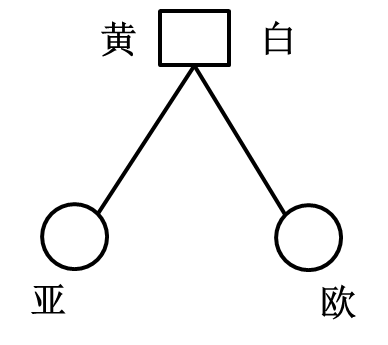
\includegraphics[width=4cm]{images/Univariate_tree.jpg}
                \caption{单变量决策树}
                \label{fig:单变量决策树}
                \end{figure}
        % \textcolor[rgb]{1 0 0}{todo:图片:单变量决策树}\\
        分类/回归问题的本质是求$y = f(x)$,不过,这里的$f$是一个特征函数$f \triangleq I_{x\in R_i}$,其中,$R_i$表示$x$的一个区域,当$x$在某个区域$R_i$内时,$y$取特定值,如图(\ref{fig:单变量决策树区域图})所示
                \begin{figure}[H]
                \centering
                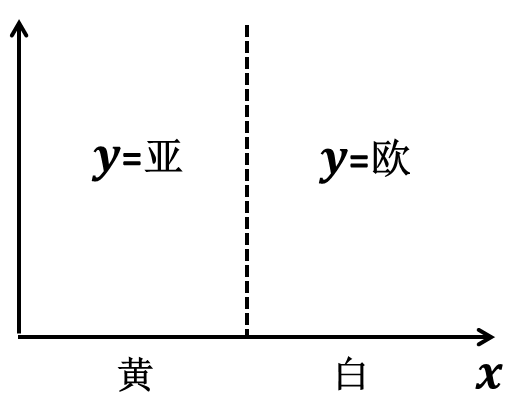
\includegraphics[width=4cm]{images/Univariate_tree_area.jpg}
                \caption{单变量决策树区域图}
                \label{fig:单变量决策树区域图}
                \end{figure}
        % \textcolor[rgb]{1 0 0}{todo:图片:单变量决策树区域图}
        \par
        将上述的离散型$x$变为连续型,则决策树区域可以是图(\ref{fig:连续型单变量决策树区域图})的情况
                \begin{figure}[H]
                \centering
                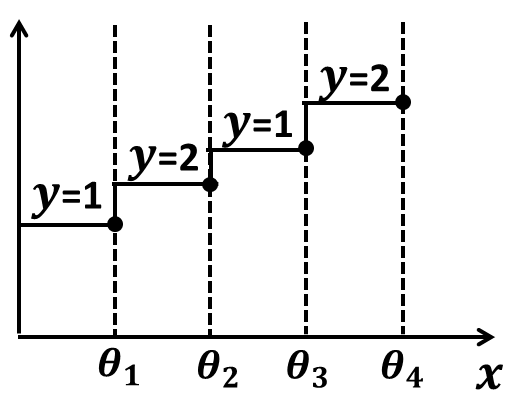
\includegraphics[width=4cm]{images/continuous_univariate_tree_area.jpg}
                \caption{连续型单变量决策树区域图}
                \label{fig:连续型单变量决策树区域图}
                \end{figure}
        % \textcolor[rgb]{1 0 0}{todo:图片:连续型单变量决策树区域图}\\
        \noindent 这里的目标是确定参数$\theta$。参数$\theta$决定了区域$R_i$从而决定了特征函数$I_\theta$。
        \par
        上面考虑的是单一变量的分类问题。下面考虑两个变量的分类/回归问题。数据类型如表(\ref{决策树两变量引例数据})所示
        \begin{table}[H]
          \caption{决策树两变量引例数据}
          \label{决策树两变量引例数据}
          \centering
          \begin{tabular}{c|ccc}
          \toprule
          data   & $x_1$(眼色)    & $x_2$(身高)    & $y$(地区) \\
          \midrule
          1      & 黑      & 中      & 亚洲 \\
          2      & 黄      & 高      & 欧洲 \\
          3      & 黑      & 中      & 亚洲 \\
          4      & 黄      & 高      & 欧洲 \\
          \bottomrule
          \end{tabular}
        \end{table}
        根据上面表(\ref{决策树两变量引例数据})的数据,可以给出地区$y$的决策树,如图(\ref{fig:两变量决策树})所示
                \begin{figure}[H]
                \centering
                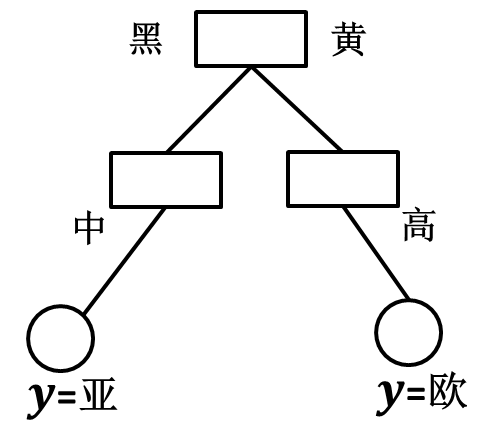
\includegraphics[width=4cm]{images/two_variate_tree.jpg}
                \caption{两变量决策树}
                \label{fig:两变量决策树}
                \end{figure}
        % \textcolor[rgb]{1 0 0}{todo:图片:两变量决策树}\\
        决策树的区域如图(\ref{fig:两变量决策树区域图})所示
                \begin{figure}[H]
                \centering
                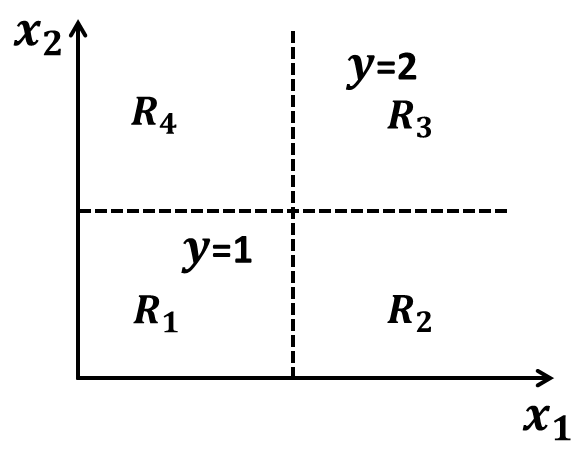
\includegraphics[width=4cm]{images/two_variate_tree_area.jpg}
                \caption{两变量决策树区域图}
                \label{fig:两变量决策树区域图}
                \end{figure}
        % \textcolor[rgb]{1 0 0}{todo:图片:两变量决策树区域图}\\
        继续考虑连续型的变量$x_1,x_2$,连续型变量的分类区域是图(\ref{fig:连续型两变量决策树区域图})的形式
                \begin{figure}[H]
                \centering
                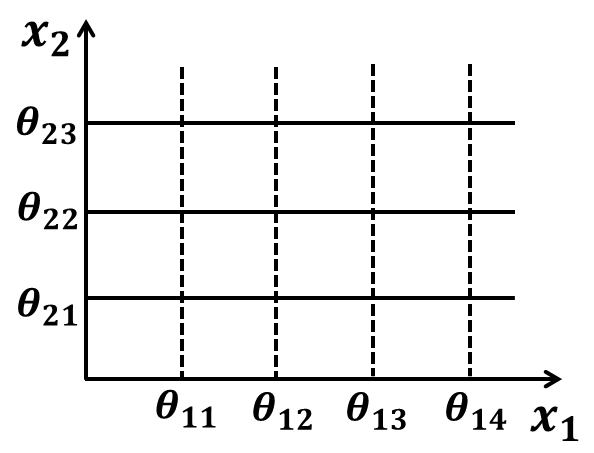
\includegraphics[width=4cm]{images/continuous_two_variate_tree_area.jpg}
                \caption{连续型两变量决策树区域图}
                \label{fig:连续型两变量决策树区域图}
                \end{figure}
        \par
        我们的目标是:确定划分区域,即确定图(\ref{fig:连续型两变量决策树区域图})中的$\theta = (\theta_1,\theta_2)$,$\theta_1 = (\theta_{11},\theta_{12},\theta_{13},\theta_{14})$,$\theta_2 = (\theta_{21},\theta_{22},\theta_{23})$。值得一提的是,虽然决策树的本质目标是求解区域参数$\theta$,但这并不是决策树的唯一目标。在建立决策树时,要先确定节点变量$x_j$,然后再确定该节点对应的参数$\theta_j$。
        \par
        将上述方法推广到多变量分类问题。设数据为$D$,共有$p$个属性变量$x_j,j=1,2,\dots,p$,变量可以是连续型、二分类、多分类和有序的。并且,设属性$x_j$的水平数为$c_j$(例如:属性“性别”的水平为“男”“女”,则其水平数为2),设变量$x_j$的参数为$\theta_j$;设标签为$y$,标签的水平数为$c_y$(这决定了是二分类问题还是多分类问题/回归问题);设共有$n$个样本。我们在数据$D$上建立决策树,将决策树模型记为$T_D$。在$T_D$中用$\square$表示属性$x_j$,称为根节点;用$\bigcirc$表示终止的分类,称为叶节点。在建立决策树$T$时,应该考虑如下问题:
        \begin{enumerate}
        \item 如何确定当前节点$x_j,j=1,2,\dots,p$?一种方法是计算$x_j$与$y$的相关性,$x_j$与上层节点的相关性,将相关性高的放在当前节点。不过要注意共线性。
        \item 如何判断该节点$x_j$的划分点(分割点)$\theta_j$?
        \item 如何判断该节点$x_j$是否需要继续划分(是否有子节点)?这是设定终止条件,可以依据当前节点下的样本数量、树深度以及当前节点下的分类正确率来判断是否终止。
        \item $x_j$可在一棵树中出现多次,能否简化?
        \item 如何添加一些外来参数$\epsilon$,使得树$T$更加灵活可调节?
        \item 如何评价树?如何评价不同的树?
        \end{enumerate}

    \subsection{基本理论}
        \subsubsection{树的生成:节点及分割点的选取}
            \par
            下面来看看ID3、ID4.5和CART等树是如何解决上面的问题(即如何生成树)。值得一提的是,对于树中叶节点上的百分数,其为条件概率,例如
            \begin{align*}
            p(y=1|x_1=1,x_2=2) = 0.97
            \end{align*}
            考虑是否有必要令$x_1,x_2$相互独立。下面来解决如何选择属性$x_j$以及如何寻找属性$x_j$的划分点/分割点$\theta_j$。
            \par
            选择划分属性(节点)及分割点$\theta$的目的是为了尽可能的区分标签,例如:
            \begin{align*}
            p(y=1|x_j <\theta_1) = 0.79\\
            p(y=1|x_j <\theta_2) = 0.83
            \end{align*}
            一般情况下,我们更愿意选择$\theta_2$作为$x_j$的分割点。接下来考虑,如何确定当前属性$x_j$,以及如何确定该属性是否需要继续划分(不满足终止条件)?在确定当前属性$x_j$时,可以使用这样一种方法:在所有属性中,将当前节点的上一层节点属性去掉,记为$\{x_j\}_-$。然后对$\{x_j\}_-$中的每一个属性$x_j$的每一种分割点$\theta_j$计算标签的区分度:条件概率$p(y=?|\cdots,x_j<\theta_j)=?$。最终,选择条件概率最大的属性$x_j$及其对应分割点$\theta_j$\footnote{注:可以想象的是,$T$是$\theta$的函数,目标是求最佳的$\theta$,使$T$“最佳”。}。这种方法本质上是一种枚举法,理论上是可行的,但并不一定实用。
            \par
            上面提到的标签区分度是条件概率(本质上就是一个概率,是样本的子样本下的一个概率),其实还有许多不同的样本区分度度量标准,例如:1.信息熵;2.信息增益(ID3);3.增益率(C4.5);4.基尼指数(CART)。
            \par
            (1)熵是信息论中的概念,用于度量系统离散程度,熵越大,系统离散程度越大。给出\underline{整个样本$D$}的熵的定义
            \begin{align*}
            Ent(D) = -\sum_{k=1}^{c_y}p_k \log_2 p_k
            \end{align*}
            其中:$p_k$为属于$k$类的概率,可以用样本的极大似然估计之,$Ent$越小,划分程度越高。上面的问题就是选择$\theta$,使样本尽可能区分开。因此,可以将熵的概念用于$\theta_j$的确定,求$\theta_j$使子样本的熵尽可能低。这里说的子样本是样本的子集,比如:样本中$x_1 = 1,x_2 = 2$的子样本。记子样本集为$D^v$,$x_j$的划分点为$\theta_{j1},\theta_{j2}$,则有
            \begin{align*}
            Ent(D^v) = -\sum_{k=1}^c p(y=k|\cdots,\theta_{j1}<x_j<\theta_{j2}) \log_2 p(y=k|\cdots,\theta_{j1}<x_j<\theta_{j2})
            \end{align*}
            称上式为在$x_j$给定后$\theta_j=(\theta_{j1},\theta_{j2})$带来的总体$D^v$的条件熵(因为是基于条件分布的)。与前面所说的条件概率相似,当$p(y=1|\cdots)=0.5$,$p(y=0|\cdots)=0.5$时,$D^v$最难分开。我们应该选择$\theta_j$使$D^v$的$Ent$尽可能小,即$p(y=k|\cdots)$尽可能大。
            \par
            (2)但不得不考虑的一个问题是样本量的偏倚,样本数量越多,影响越大。定义信息增益(information gain)为
            % \textcolor[rgb]{1 0 0}{todo:公式:有问题}
            \begin{align*}
            Gain(D)_{\theta_j} = Ent(D) - \sum_{v=1}^{\mathrm{num}_{\theta_j}}\frac{|D^v|}{|D|}Ent(D^v)
            \end{align*}
            此Gain为ID3算法选择属性$x_j$和分割点$\theta_j$的策略。
            \par
            (3)虽然上面的Gain解决了样本量的偏倚,但应该注意到会有表(\ref{子样本的特殊情况})这种情况
            \begin{table}[H]
            \caption{子样本的特殊情况}
            \label{子样本的特殊情况}
            \centering
            \begin{tabular}{l|ll}
            \toprule
            $D^v$   & $x_j$    & $y$   \\
            \midrule
            1      & 1      & 0   \\
            2      & 2      & 1   \\
            3      & 3      & 0  \\
            4      & 4      & 1   \\
            5      & 5      & 0   \\
            \bottomrule
            \end{tabular}
            \end{table}
            如果$x_j$的分割点$\theta_j = (1,2,3,4,5)$,则每个$p(y=\cdot|\cdot<x_j<\cdot)$仅含有一个样本,这会导致其不具有推广能力。为此,Quinlan于1993年设置了C4.5(商用版本为C5.0)的增益率(gain ratio)
            \begin{align*}
            Gain\_ratio(D)_{\theta_j} = \frac{Gain(D)_{\theta_j}}{IV_{\theta_j}}
            \end{align*}
            其中:
            \begin{align*}
            IV_\theta = -\sum_{v=1}^{\mathrm{num}_{\theta_j}}\frac{|D^v|}{|D|}\log_2\frac{|D^v|}{|D|}
            \end{align*}
            \par
            (4)基尼指数。另外,Breiman在1984年开发的CART树是通过基尼指数来进行选择。Gini定义为
            \begin{align*}
            Gini(D) = 1-\sum_{c=1}^{c_y}p^2(y=k)
            \end{align*}
            Gini反映了从数据集$D$中随机抽取两个样本,其标签不同的概率。对于子样本,$Gini(D^v)$定义为
            \begin{align*}
            Gini(D^v)_{\theta_j} = 1-\sum_{k=1}^{c_y} p^2(y=k|\cdots,\theta_{j,i}<x_j<\theta_{j,i+1})
            \end{align*}
            进一步考虑样本量的影响,有
            \begin{align*}
            Gini\_index(D)_{\theta_j} = \sum_{v=1}^{\mathrm{num}_{\theta_j}}\frac{|D^v|}{|D|}Gini(D^v)
            \end{align*}
            于是,我们要选择$\theta_j$使得$Gini\_index(D)_{\theta_j} $尽可能小,有
            \begin{align*}
            \theta_j^* = \arg\min_{\theta_j\in \Theta}\ Gini\_index(D)_{\theta_j}
            \end{align*}
        \subsubsection{树的修剪}
            \par
            决策树已经建好了吗?并没有,前面所做的工作只是介绍了树的生长方式:如何选择节点$x_j$以及分割点$\theta_j$。这些工作可以生成一棵枝繁叶茂的树,但并不一定是一棵“漂亮”的树。在经过一系列的生长后,到了用$x_j$划分的时候,发现$x_j$下的子样本仅有几个。出现这种情况的原因是:\ding{172}属性节点太多;\ding{173}样本量太少。这种树会导致过拟合现象,为此,有必要考虑一下“园丁”的工作:修剪树枝(去掉一些节点属性)。根据上述情况产生的原因\ding{172}和\ding{173},我们可以规定:
            \begin{enumerate}
            \item 属性达到一定的数目后就不再生长,即当树的根节点达到一定数目时就不再生长。设定数目阈值为$\epsilon_1$;
            \item 子样本数目小于一定数目时就不再生长。设定子样本最小数目为$\epsilon_2$;
            \end{enumerate}
            其中:$\epsilon_1,\epsilon_2$就是我们前面所说的外来参数。它们是人为添加的,用于控制树$T$的生长。但这种方法是人为设置的,有很强的主观性,有可能导致该出现的枝未出现。一般书上称这种工作为“预剪枝”,其实,这并不能称为剪枝,而应该称为抑制生长。
            \par
            对“应该出现的分枝未出现”,也可以有相应的改进策略,我们让所有的枝都生长出来,看枝的“价值”如何,然后将价值低的枝减掉。一般书上称此策略为“后剪枝策略”。那么,问题来了:枝是什么?如何评价枝的价值?如何剪枝?
            \par
            C4.5使用的是悲观剪枝法,CART使用的是代价复杂度剪枝法。下面来介绍这两种剪枝方法。我们称树$T$的一部分为树枝,如图(\ref{fig:决策树树枝示意图})所示
                \begin{figure}[H]
                \centering
                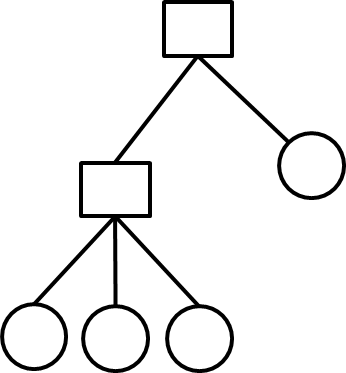
\includegraphics[width=3cm]{images/Decision_tree_branches.jpg}
                \caption{决策树树枝示意图}
                \label{fig:决策树树枝示意图}
                \end{figure}
            % \textcolor[rgb]{1 0 0}{todo:图片:决策树树枝示意图}\\
            设节点$t$下的树枝为$T_t$,节点$t$(注意,这里的节点为叶节点,如果我们将某一根节点下的叶节点剪枝,则该根节点变为叶节点)的错误率为$e_t$,样本数$N_t$,错误样本数$E_t$。错误率,即新来样本在子节点处被判错的概率。如果所有子节点下的加权错误率大于父节点,则去掉这些子(叶)节点。
            \par
            C4.5是从底层开始逐层向上修剪,关键问题是误差的估计以及修剪标准的设置。考虑如下图(\ref{fig:C4.5决策树})的决策树
                \begin{figure}[H]
                \centering
                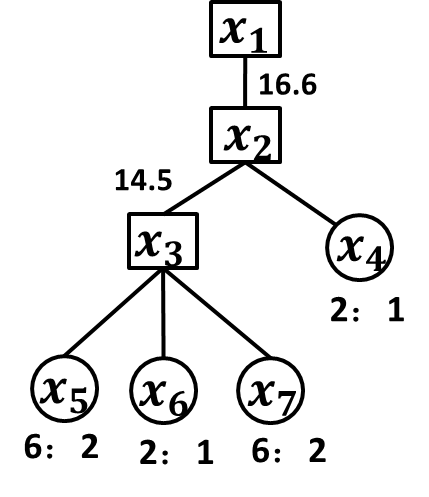
\includegraphics[width=4cm]{images/C4.5.jpg}
                \caption{C4.5决策树}
                \label{fig:C4.5决策树}
                \end{figure}
            % \textcolor[rgb]{1 0 0}{todo:图片:C4.5决策树}\\
            \noindent 其中:各节点下的数字比例$?:?$表示:前一个数字为该节点$t$下的样本数$N_t$,后一个数字为错判样本数$E_t$。例如:在(叶)节点$x_7$处终止,有6个子样本,其中4个为1,2个为0。但现在终止了,也就说明对于一个新来样本,在该处会被判为1。节点$t \triangleq x_7$的错误率为$\hat{e}_t= \frac{E_t}{N_t} = \frac{2}{6}$。$\hat{e}_t$的本质是一个样本估计量。然后来说明C4.5中“悲观”所在。其实,悲观是指在置信水平$\alpha$下,错误率$e_t$的估计上限
            \begin{align*}
            \hat{e}_t = \frac{E_t}{N_t}+Z_{\frac{\alpha}{2}}\sqrt{\frac{\frac{E_t}{N_t}(1-\frac{E_t}{N_t})}{N_t}}
            \end{align*}
            注:这里有
            \begin{align*}
            \frac{\frac{E_t}{N_t} - e_t}{\sqrt{\frac{\frac{Et}{N_t}(1-\frac{E_t}{N_t})}{N_t}}} \overset{\cdot}{\sim } N(0,1)
            \end{align*}
            当子节点$(x_5,x_6,x_7)$的加权错误率超过父节点$x_3$的错误率,则去掉子叶节点$x_5,x_6,x_7$,根节点$x_3$变为叶节点。
            \par
            当然,还可以通过其它手段来体现悲观。考虑如图(\ref{fig:用于悲观剪枝法的两个树枝})两个树枝$T_L,T_R$($T_L$剪掉下层叶节点变为$T_R$)
            	\begin{figure}[H]
  				\centering
  				\begin{varwidth}[t]{\textwidth}
    			\vspace{0pt}
    			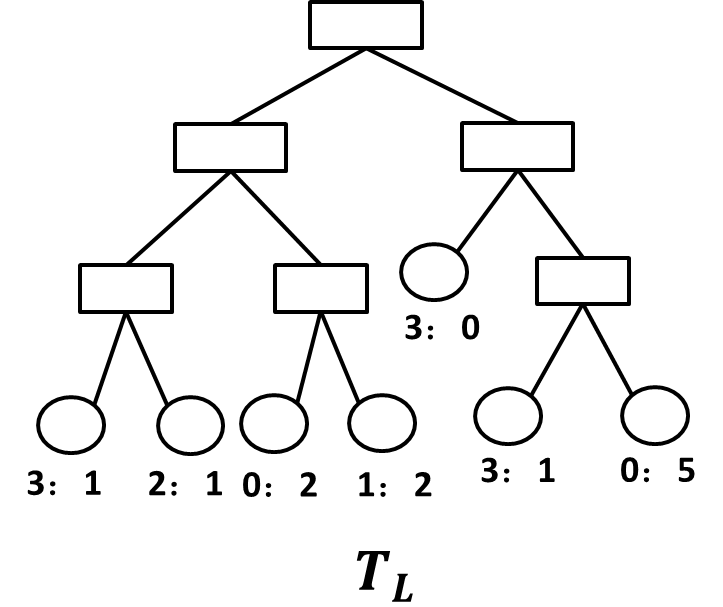
\includegraphics[height=4cm]{images/Two_branches_for_pessimistic1.png}
  				\end{varwidth}
  				\qquad \qquad
  				\begin{varwidth}[t]{\textwidth}
    			\vspace{0pt}
    			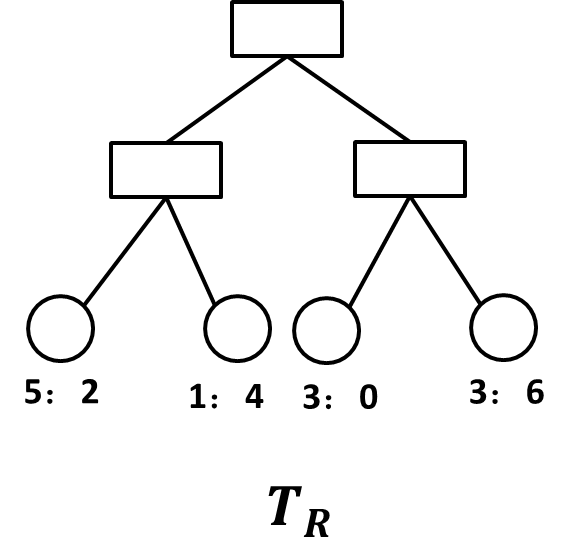
\includegraphics[height=4cm]{images/Two_branches_for_pessimistic2.jpg}
  				\end{varwidth}
				\caption{用于悲观剪枝法的两个树枝}
				\label{fig:用于悲观剪枝法的两个树枝}
				\end{figure}
            % \textcolor[rgb]{1 0 0}{todo:图片:用于悲观剪枝法的两个树枝}\\
            上图(\ref{fig:用于悲观剪枝法的两个树枝})中的叶节点处的数值比表示为\underline{真假样本比例}。定义树枝的悲观度为
            \begin{align*}
            e_g(T_t) = \frac{\sum_{i=1}^k(E_{t_i}+\Omega_{t_i})}{\sum_{i=1}^k N_{t_i}} = \frac{E(T_t)+\Omega(T_t)}{N_t}
            \end{align*}
            其中:$t_i$为叶节点,$E_{t_i}$为叶节点$t_i$下的错误样本,$N_{t_i}$为叶节点$t_i$下的总样本,$\Omega_{t_i}$为叶节点$t_i$的惩罚, $k$为枝$T_t$的叶节点数,$T_L$的叶节点数为7,$T_R$的叶节点数为4;设每个叶节点$t_i,i=1,2,\dots,k$的惩罚为0.5,则有
            \begin{align*}
            e_g(T_L) = \frac{4+7\times 0.5}{24}=0.3125\\
            e_g(T_R) = \frac{6+4\times 0.5}{24} = 0.3533
            \end{align*}
            \par
            上面介绍了C4.5的悲观剪枝法,下面来介绍CART的代价复杂性剪枝法。C4.5的悲观剪枝法对枝的价值是通过下面的错判误差来衡量的,且由于是由下层逐层向上计算,枝也仅包含2层。而CART对枝价值的评价不仅仅包含2层,而是更多层。我们记CART的枝的价值为$R$,$R$价值\uline{同样是由错误率与复杂性度量的},与C4.5不同的是,其错误率是在测试集上计算的。定义枝$T$的价值/代价复杂度为
            \begin{align*}
            R_\alpha(T) = R(T)+\alpha(|T| - 1)
            \end{align*}
            其中:$R(T)$为$T$在测试集上的误差,$|T|$表示枝$T$的子节点数目(去掉父节点的),$\alpha$为复杂度系数,表示每增加一个子节点带来的复杂度。CART的修剪步骤为:\\
            \textbf{Step1.}对于最大的树$T_1$,令$\alpha=0$,计算复杂度,不断增加$\alpha$,直到有一个子枝可以被剪掉,此时得到子树$T_2$。这里介绍剪掉内部节点$t$的分枝的方法:当$\alpha \geqslant \frac{R(t)-R(T_t)}{|T_t-1|}$时,内部节点$\{t\}$的代价复杂度小于等于子树$T_t$,则可以剪掉内部节点$t$的分枝。\\
            \textbf{Step2.}重复步骤1,直到剩下最后一个根节点。最终得到的子树序列为$\{T_1,T_2,\dots,T_k\}$及它们的代价复杂度$R_\alpha(T_1),R_\alpha(T_2),\dots,R_\alpha(T_k)$。\\
            \textbf{Step3.}确定最终修剪结果$T_{opt}$
            \begin{align*}
            R(T_{opt}) \leqslant \min_k \ R(T_k) + m SE(R(T_k))
            \end{align*}
            其中:$m$为放大因子,$SE(R(T_k))$为子树$T_k$在测试集上的预测误差的标准误
            \begin{align*}
            SE(R(T_k)) = \sqrt{\frac{R(T_k)(1-R(T_k))}{N_t}}
            \end{align*}
            \par
            这里,我们详细说明一下Step1。如图(\ref{fig:CART剪枝示意图})所示
            	\begin{figure}[H]
  				\centering
  				\begin{varwidth}[t]{\textwidth}
    			\vspace{0pt}
    			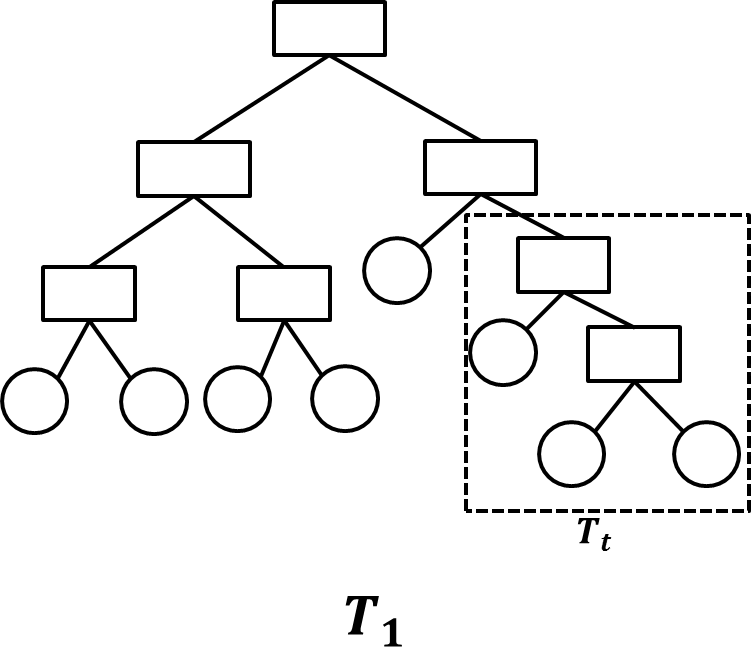
\includegraphics[height=4cm]{images/CART1.jpg}
  				\end{varwidth}
  				\qquad \qquad
  				\begin{varwidth}[t]{\textwidth}
    			\vspace{0pt}
    			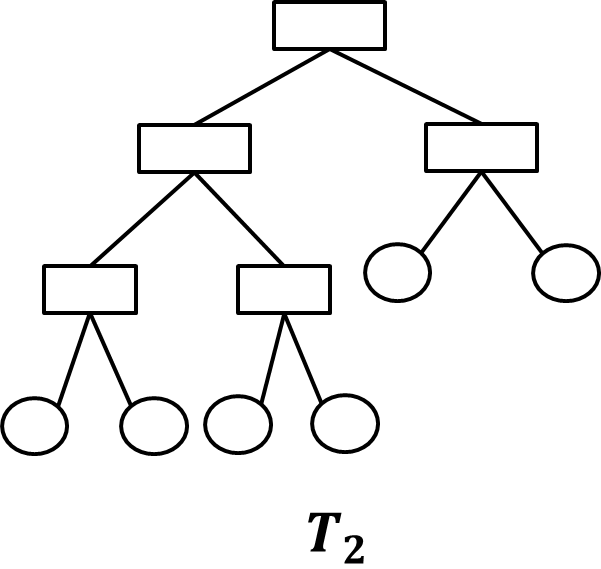
\includegraphics[height=4cm]{images/CART2.jpg}
  				\end{varwidth}
                \caption{CART剪枝示意图}
                \label{fig:CART剪枝示意图}
				\end{figure}
            % \textcolor[rgb]{1 0 0}{todo:图片:CART剪枝示意图}\\
            计算完全树$T_1$的代价复杂度$R_\alpha(T_1),\alpha = 0$;令$\alpha = \alpha+1$,判断$T_1$中是否有子枝可以被剪,比如:针对图(\ref{fig:CART剪枝示意图})中的节点$t$和枝$T_t$而言,对$R_\alpha(t)$的复杂度和$R_\alpha(T_t)$的复杂度进行计算
            \begin{align*}
            & R_\alpha(t) = R(t)+\alpha \\
            & R_\alpha(T_t) = R(T_t)+\alpha(|T| - 1)
            \end{align*}
            其中:$R(t)$是将测试集带入到树$T$中,只计算到$t$节点时的错误率;$R(T_t)$是将测试集带入到树$T$中,计算到最后,$T_t$的错误率。
            当$\alpha \geqslant \frac{R(t)-R(T_t)}{|T_t-1|}$时,剪掉$T_t$枝。
            \par
            下面介绍ID3、C4.5、CART、CHAID和QUEST树的应用范围。(1)C4.5可以用于建立多叉分类树,要求输入变量是分类型/连续型,输出变量是分类型,以信息率为建树准则,以悲观误差估计为剪枝策略,不用测试集。(2)CART只能建立二叉树,要求输入变量是分类型/连续型,输出变量为分类型/连续型,Gini系数作为建树准则,以代价复杂性作为剪枝准则,需要测试集。(3)CHAID称为卡方自动交互诊断器,由Kass于1980年提出,可以建立多叉树,输入和输出变量可以是连续型/分类型,它以卡方统计显著检验作为建树准则,以相关性限定策略作为剪枝策略。(4)QUEST是由Loh和Shih于1997年提出,可建立二叉树,要求输入变量是分类型/连续型,输出变量为分类型,它以统计方法为基础进行建树。

        \subsubsection{树的评估}
            \par
            在前面的CART的剪枝策略中,我们构建了$\{T_1,T_2,\dots,T_k\}$棵树,然后选择了$T_{opt}$,这种剪枝的本质是用CART策略生成不同的树,然后从中选择最好的。并且,对于同一个数据集$D$,我们可以建立不同的树,那么如何评价这些树对于我们的问题/$D$的好坏呢?很自然想到,如果新来一批样本(测试集),哪棵树的误差小,那棵树就是好的。这里,我们是用误差作为树优良的评判标准,同样,还有提升度,收益率等评判标准。先来泛化误差的计算。为了体现泛化,我们有必要构造不同的数据集$D_1,D_2,\dots,D_k$,并在这些数据集上测试模型。下面介绍几种可行的,通过$D$来构造$\{D_k\}$的方法:
            \par
            (1)保持法:使用训练集和检验集(非测试集),在检验集上计算平均准确率,如果计算总准确率,最好使不同模型的检验集样本数目相同。但是这种方法受样本量的限制。
            \par
            (2)随机(二次)采样:从$D$中随机抽取样本,设每次采样数目为$n_1,n_2,\dots,n_k$(共有$k$次采样,形成$k$个样本),用$i$作为标记,$acc_i$是第$i$次抽样的准确率
            \begin{align*}
            acc_i = \frac{E_i}{n_i}
            \end{align*}
            则总采样准确率为
            \begin{align*}
            acc_{sub} = \sum_{i=1}^k\frac{acc_i}{n_i}
            \end{align*}
            平均准确率为
            \begin{align*}
            acc_{avg} = \frac{acc_{sub}}{\sum_{i=1}^kn_i}
            \end{align*}
            \par
            问:随机采样是真的从$D$中再生成子样本,但其子样本已经参与过建树的过程(检验集中的样本则没有参与建树过程),这样的话能用其充当新样本吗?其实,建树过程只用了该样本的部分信息,有些信息在修剪的过程中被剪掉了。
            \par
            (3)$k$折交叉验证:在$k$折交叉验证中,我们将样本集分为$k$个子集,先用第一个子集作为检验集,剩下的子集作为训练集进行训练,得到误差$e_1$,然后用第二个子集作为检验集,剩下的子集作为训练集进行训练,得到误差$e_2$,如此反复,直到第$k$个子集作为检验集,得到$e_k$。最终的误差为$e = \sum_i e_i$。
            \par
            (4)bootstrap技术(自助法):自助法是估计一个统计量均值、方差和分布的一种有效的方法。并且这种方法是有放回抽样。设有$n$个训练样本,设定有放回法采样$k$次,每次采样量为$\alpha_i$,$\alpha_i$可以相同,也可以不同。用$i$作为次数标记,$acc_i$为第$i$次有放回采样的准确率,则bootstrap方法的准确率为
            \begin{align*}
            acc_{boot} = \frac{1}{k}\sum_{i=1}^k \left( \frac{\alpha_i}{n} \frac{E_i}{\alpha_i}+(1-\frac{\alpha_i}{n})acc_i\right)
            \end{align*}
            \par
            上面介绍了用于模型评价的泛化误差的计算,对于分类模型的评价,还可以采用混淆矩阵、ROC曲线、提升度和收益率等。
    \subsection{MATLAB应用实例}
        \par
        MATLAB中使用fitctree函数来实现决策树的创建,其调用格式为tree = fitctree(x,y,Name,Value);使用cvloss来实现决策树剪枝,其调用格式为
        \par
        [~,~,~bestlevel] = cvloss(tree,'subtrees','all','treesize','min')
        \par
        cptree = prune(tree,'Level','bestlevel')
        \par
        用resubloss来计算重带入误差,用kfoldloss来计算交叉验证误差,用predict来进行预测。下面给出一个简单的MATLAB应用实例
        \begin{lstlisting}[language = Matlab]
        tree = fitctree(means(:,1:2),species,'PredictorNames',{'sl','sw'});%创建决策树
        [grpname,node] = predict(tree,[x,y]);
        %绘制混淆矩阵
        targetoutput = y';
        output = predict(model_tree_Y1,X_tree_test); output = output';
        targetoutput = full(ind2vec(targetoutput+1));
        output = full(ind2vec(output+1));
        plotconfusion(targetoutput,output);
        clear output
        gsscatter(x,y,grpname,'grb','sod')
        view(tree,'model','graph')%绘制决策树
        dtResabErr = resubloss(tree);%重带入误差
        crt = crossval(tree, 'CVPartitin', 'cp');
        dtCVErr = kfoldloss(crt);%k折交叉验证误差
        resubcost = resubloss(tree,'subtrees','all');
        [cost,secost,ntermnodes,bestlevel] = cvloss(tree,'subtrees','all')%计算最优level
        plot(ntermnodes,cost,'b-',ntermnodes,resubcost,'r--')
        figure(gcf)
        xlabel('Number of terminal nodes')
        ylabel('cost misclasification error')
        legend('Cross-ralidation','Resubstitation')
        [mincost,minloc] = min(cost)
        cutoff = mincost + secost(minloc)
        hold on
        plot([0,20],[cutoff cutoff], 'k:')
        plot(ntermnodes(bestlevel+1), cost(bestlevel+1),'no')
        legend('Cross-ralidation','Resubstitation','Min+1 ster.err','Best cloice')
        hold off
        pt = prune(tree,'level','best level')%决策树剪枝
        view(pt,'mode','graph')
        cost(bestlevel+1)
        %查看树
        % treetype = type(tree)
        % var6 = cutvar(tree,6) % 该节点是什么变量
        % type6 = cuttype(tree,6) % 变量是什么类型
        \end{lstlisting}

\section{集成学习}
    \subsection{引言}
        \par
        常用的集成学习有两种:Boosting(提升方法)和Bagging(打包方法)\cite{1999.Bauer}\cite{2000.Dietterich}。Boosting族是一种可将弱分类器提升为强分类器的学习方法,有Adaboost等;Bagging是一种基于bootsrtap方法的集成建模方法,有RandomForest(随机森林)等。这里,我们先来介绍两种集成学习方法的不同之处,之后,再详细介绍boosting方法。Bagging对训练集进行随机抽样,并且各轮训练相互独立,最终的预测函数没有权重,易于并行训练;而boosting方法的各轮训练并不相互独立,当前训练与前一轮训练的误差密切相关,并且boosting方法的预测函数有权重,只能顺序生成。在大多数数据集上,boosting的准确率要比bagging更高。
        \par
        Boost方法被放在了机器学习部分的最后,在前面的机器学习部分,我们介绍了许许多多的分类/回归(预测)方法,这些方法都可以作为Boost方法的简单分类器。Boost方法和组合预测的思想类似,对于同一个分类/回归数据,我们用不同的模型(弱分类器)进行分类,然后将这些模型的结果综合(评价),形成最终的分类结果。我们前面提到过,基本的MLP(多层感知器)就是线性回归的组合策略。下面,我们要考虑的问题是:如何选择单一的分类模型?模型参数如何调整?如何组合分类结果?
        \par
        如何将多个分类器的分类结果组合,或者更详细的说,对于具体的某一样本$x^k$,我们有$M$个分类器的结果$y_1^k = 1,y_2^k = 3,y_3^k = 1,\dots,y_M^k = 1$,那么,这个样本$x^k$的类别最终应判为哪一类呢?我们自然想到,用$M$个分类结果的众数来作为最终的判别结果,如果对回归预测而言,就用$M$个回归模型预测的均值作为最终预测结果,这种思想被称为committee(委员会)。
        \par
        我们有必要先研究一下这个组合估计的均值和方差大小,并与单一分类器得到的均值方差进行比较。当然,后面介绍的Boost方法也要讨论估计量的性质。boosting方法是committee方法的变体,boosting方法有3种基本的结构:
        \begin{enumerate}
        \item 通过过滤推举:用一个弱学习算法的不同版本过滤训练样本,有些样本在训练过程中会被抛弃,有些则保留,这个方法要求样本量大,但它需要的存储空间较小。
        \item 通过子抽样提升:这种方法用到一个固定大小的训练样本,训练中这些样本以一定的概率(权重)被重新抽取。
        \item 通过加权推举:这种方法也用到一个固定大小的训练样本,但他决定弱学习算法能接收加权后的样本。
        \end{enumerate}
        \subsubsection{Committee}
            \par
            无论对于分类问题还是回归问题,仍假设我们得到的样本集为$S=\{x^k,y^k\}_{k=1}^m,x^k = (x_1^k,x_2^k,\\\dots,x_n^k)$,$S\subset R^n$,$y^k\in R$或者$\{1,2,\dots,c\}$。为了描述方便,这里我们考虑回归问题,我们要在样本集上建立$M$个回归模型,然后将这些模型的结果综合,给出最终的预测/估计。假设第$i$个模型的回归估计值为$y_i = (y_i^1,y_i^2,\dots y_i^m)$,$M$个回归模型的估计做平均,有
            \begin{align*}
            y(x) = \frac{1}{M} \sum_{i=1}^M y_i(x)
            \end{align*}
            \par
            下面来分析这个估计量$y(x)$的均值和方差。设第$i$个模型$y_i(x)$的误差为$\varepsilon_i(x)$,有离差平方和
            \begin{align*}
            \mathbb{E}_x[(y-y_i(x))^2] = \mathbb{E}_x[\varepsilon_i(x)^2]
            \end{align*}
            其中:$y$为样本真实输出,$y_i(x)$为估计。于是,各模型独立预测时的平均误差为
            \begin{align*}
            E_{arg} = \frac{1}{M} \sum_{i=1}^M \mathbb{E}_x[\varepsilon_i(x)^2]
            \end{align*}
            类似的,Commttee方法的期望误差/平均误差为
            \begin{align*}
            E_{com} &= \mathbb{E}_x[(y(x)-y)^2]\\
            &=\mathbb{E}\left[\left(\frac{1}{M}\sum_{i=1}^M y_i(x)-y\right)^2\right]\\
            &=\mathbb{E}_x\left[\left( \frac{1}{M} \sum_{i=1}^M \varepsilon_i(x) \right)^2   \right]
            \end{align*}
            如果我们假设
            \begin{align*}
            & \mathbb{E}_x[\varepsilon_i(x)] = 0\\
            & \mathbb{E}_x[\varepsilon_i(x)\varepsilon_j(x)] = 0
            \end{align*}
            则有
            \begin{align*}
            E_{com} = \frac{1}{M}E_{arg}
            \end{align*}
            \par
            这个结果表明:对一个模型而言,可以通过模型的$M$个版本求平均(组合)的方式,使误差减小$M$倍。但是,这个结果依赖于前面的假设,即由单个模型产生的误差是不相关的,但在实际中,误差间往往高度相关。幸运的是,我们仍能证明组合策略的一大特点是
            \begin{align*}
            E_{com} \leqslant E_{arg}
            \end{align*}
            即组合分类/预测模型的期望不会超过单一模型的期望。
    \subsection{Boosting起源}
        \par
        Boosting方法是一种非常强大的方法,它将多个弱分类器进行组合,产生新的强分类器,强分类器比任何一个弱分类器都要好。
        Boosting方法几乎可以应用到前面介绍的各种分类方法当中(应该也可以应用到聚类方法)。Boosting打破了原样本的分布,这一点是至关重要的。下面,我们将要描述:1.PAC和Boosting猜想及证实以及Boosting最初的设计;2.Adaboost训练误差及泛化误差;3.几种重要的Adaboost理论分析模型,并由此引出一些AdaBoost的改进;4.介绍AdaBoost从二分类到多分类即回归问题的推广。
        \par
        在可能近似正确(Probably approximately Correct, PAC)学习框架中,$X$是样本空间,$C$是目标种类集,$C$中的每一个元素$c$对应着$X$上的某一个子集,$D$是样本空间$X$的固定但未知的分布函数,训练集$S = \{x^k\}_{k=1}^m$是从分布$D$中独立随机抽取的样本集。
        \par
        现在,假设有一个分类器$f(x)$,分类器$f(x)$在样本$x$上的错误率为$e(f) = P_{x\in D}[c(x) \neq f(x)]$,PAC学习模型弱化对分类器$f(x)$的要求,不要求$f(x)$输出其错误率,只要错误率在一个很小的常数$\varepsilon$内,不要求$f(x)$对任何随机抽取的训练样本都能成功,只要失败的概率在一个很小的$\delta$内即可。
        \par
        定义PAC的强学习概念:考虑一个$n$分类问题,$C=\{1,2,\dots,n\}$,有一训练集$S$,$\forall c\in C$、$S$上的任意样本分布$D$、$0<\varepsilon <\frac{1}{2}$、$0<\delta<\frac{1}{2}$,如果存在$\frac{1}{\varepsilon},\frac{1}{\delta},n$和$size(c)$的多项式复杂度的算法A,能够以$1-\delta$的概率输出假设$f$,且$f$的错误率$e(f) \leqslant \varepsilon$,则称类$c$是PAC强可学习的,称算法A是一个强学习算法。
        \par
        如果只需要存在某对$\varepsilon,\delta$,使得以上结论成立,则类$c$是PAC弱可学习的,称算法A为弱学习算法。
        \par
        1989年,Kearns和Valiant在研究PAC时提出\cite{1984.Valiant}:弱可学习是否等价于强可学习?如果等价,那么任意给定一个仅比随机猜测好的弱学习算法(准确率$>0.5$),可以通过加强提升到一个任意准确率的强学习算法,并可以通过构建一个多项式级的算法来实现这一加强(提升)过程,这使得我们不必直接去寻找难以构建的强学习算法。Schapiro通过构造性方法证明:一个类是弱可学习的,当且仅当它是强可学习的。其构造过程如下:\ding{172}首先依分布$D$产生训练集$S$的一个子集$EX_1$,调用算法weaklearn得到分类器$f_1$,只要分类器$f_1$是一个弱分类器;\ding{173}接着,构造样本集$EX_2$,其一半是被$f_1$正确分类的样本,一半是错误分类的样本,训练得到分类器$f_2$;\ding{174}最后,选择$f_1,f_2$分类结果不同的样本构成$EX_3$,调用weaklearn训练得到分类器$f_3$;\ding{174}对新样本,由$f_1,f_2,f_3$投票决定。可以证明,若$f_1,f_2,f_3$在任意分布下的错误率$\alpha$5均小于$\frac{1}{2}$,则$f = \mathrm{sgn}(f_1+f_2+f_3)$在任意分布下的错误率$g(\alpha) \leqslant 3\alpha^2-2\alpha^3$。这意味着上述算法可以得到一个更低错误率的分类器$f$,并且,如果继续深入上述算法,最终分类器$f$的错误率可以任意低。强学习算法如(\ref{code:强学习算法})所示
        \begin{algorithm}[H]
            \caption{强学习算法Learn}\label{code:强学习算法}
            \begin{algorithmic}[1]
                \State 初始化:训练样本集$EX$,弱学习算法weaklearn,weaklearn的错误率上界$\varepsilon$,置信度$\delta$。
                \State 如果$\varepsilon \geqslant (1/2 - r)$,返回weaklearn(EX);
                \State $\alpha = g^{-1}(\varepsilon)$;
                \State $f_1 = learn(\alpha,\delta/k,EX_1)$;
                \State $f_2 = learn(\alpha,\delta/k,EX_2)$;
                \State $f_3 = learn(\alpha,\delta/k,EX_3)$;
            \end{algorithmic}
        \end{algorithm}
        \par
        注意到,上述强学习算法要求弱学习算法weaklearn的误差率$\varepsilon$满足一定要求,并且,在构建$f_1,f_2,f_3$时,误差置信度是$1-\delta/k$,最终分类器$f$的置信度为$(1-\delta/k)^k > 1-\delta$。算法每次递归的性能增益与最大错误率$\varepsilon$称多项式关系,所以递归层数是多项式复杂性的,至此,证明了弱学习算法可以被提升到以$1-\delta$概率输出错误率小于任意$\varepsilon$的假设(即强学习算法)。上述过程打破了分类器在已有样本上的优势,重新采样使接下来的分类器聚焦于难分类的样本。然而,由于算法要求我们提前预知弱分类器的错误率上界$\varepsilon$,因此,在实际中上述算法很难应用。
    \subsection{AdaBoost算法}
        \par
        1995年Freund\cite{1995.Yoav}提出Adaboost算法。Freund和Schapire发现,在线分配问题与Boosting问题之间存在着很强的相似性,引入在线分配算法的设计思想,有助于设计出更实用的boosting算法。我们将加权投票的相关研究成果与在线分配问题结合,并在Boosting问题框架下进行对应推广,得到了著名的Adaboost算法。Adaboost算法不再要求预先知道弱学习算法weaklearn的任何先验知识,在实践中取得了巨大的成功。
        \par
        AdaBoost的主要步骤为:首先给出弱分类器和样本集$S = \{x^k,y^k\}_{k=1}^m$,每个样本都赋予一个权重$w^k,k=1,2,\dots,m$,设初始权重$w^k_0 = \frac{1}{m}$;然后,我们用弱学习算法迭代$M$次,每次运行结束后,都按照分类结果的准确性更新样本权重,对于分类失败的训练样本赋予较大的权重,下次迭代训练时,有较大机会挑选到失败的样本。我们在每一个$i(i=1,2,\dots,M)$都得到了一个分类器$f_i(i=1,2,\dots,M)$,将这$M$个分类器按照一定权重组合,结果准确率高的分类器赋予大的权重,最终形成的强分类器$F$。AdaBoost算法步骤如下:\\
        \textbf{Step1.}初始化。$S=\{x^k,y^k\}_{k=1}^m$,弱分类器$f$可以选择SVM或BP或决策树等,$M$,$i: = 0$,$w^k_0 = \frac{1}{m}$。\\
        \textbf{Step2.}对$i=0,1,\dots,M-1$训练第$i$个分类器$f_i$:
        \par
        \ding{172}对$x_i$进行训练,得到分类器$f_i(x)$。分类器的目标是最小化加权误差
        \begin{align*}
        J_i = \sum_{k=1}^m w^k_i I_{f_i(x^k) \neq y^k}
        \end{align*}
        其中:$I$是特征函数,$f_i$表示第$i$次的分类器,$x^k$为第$k$个样本。
        \par
        \ding{173}计算$\epsilon_i,\alpha_i$
        \begin{align*}
        & \epsilon_i = \frac{J_i}{\sum_{k=1}^m w_i^k} = \sum_{k=1}^m \frac{w_i^k}{\sum_{k=1}^m w_i^k} I_{f_i(x^k)\neq y^k}\\
        & \alpha_i = \frac{1}{2}\ln \left( \frac{1-\epsilon_i}{\epsilon_i} \right)
        \end{align*}
        $\epsilon_i$是加权错误率且$\sum_{k=1}^m w_i^k \neq 1$。
        \par
        \ding{174}更新样本的权重$w_{i+1}^k$
        \begin{align*}
        w_{i+1}^k = w_i^k \exp\{\alpha_i I_{f_i(x^k)\neq y^k}\}
        \end{align*}
        被分错的样本$k$的权重$w^k$会变大,分对的样本的权重保持不变$(\exp(0)=1)$。\\
        \textbf{Step3.}终止条件。如果不终止,则置$i:=i+1$,返回Step2;终止后,输出最终的组合分类模型
        \begin{align*}
        F(x) = \sum_{i=1}^M \alpha_i f_i(x)
        \end{align*}
        \subsubsection{AdaBoost的误差分析}
            \par
            (1)训练误差。我们先来看AdaBoost的训练误差,在AdaBoost提出之初,Freund就分析了AdaBoost的训练误差。Freund等在1995年的原文中首次证明:若Adaboost每一轮迭代中生成的子分类器错误率分别为$\varepsilon_1,\varepsilon_2,\dots,\varepsilon_M$,则组合分类器$F = \sum_{i=1}^M\alpha_i f_i$的训练错误率$\varepsilon$有上界:$\varepsilon \leqslant 2^M \prod_{i=1}^M \sqrt{\varepsilon_i(1-\varepsilon_i)}$。
            \par
            随后,Schapire等又给出另一种更简单的误差界推导方法,得到
            \begin{align*}
            \varepsilon = \frac{1}{m}\sum_{k=1}^m [F(x^k)\neq y^k] \leqslant \frac{1}{m}\sum_{k=1}^m\exp \left( -y^k\sum_{i=1}^M \alpha_i f_i(x^k) \right)  = \prod_{i=1}^M z_i
            \end{align*}
            其中:$z_i$是第$i$轮迭代的样本归一化因子
            \begin{align*}
            z_i = \sum_{k=1}^m w_i^k \exp (-\alpha_iy^k f_i(x^k))
            \end{align*}
            $w_i^k$是样本$x^k$在第$i$次迭代中的样本权重。
            \par
            上面给出了AdaBoost的训练误差界,但是这种误差界过于宽松,在实际训练中,AdaBoost的表现要比这个误差界好很多。虽然过于宽泛,但该过程可以用来指导我们寻找单一分类器$f_i(x)$。我们只要找到$f_i(x)$及$\alpha_i$使$\prod_{i=1}^M z_i$最小,即可得到高精度的强分类器$F$。然而,$\min\prod_{i=1}^M z_i$的全局最小化,每加入一个新的子分类器,都可能需要修改已有的子分类器,这样做的话训练复杂度会很高。为了避免这个复杂的优化问题,AdaBoost使用贪心策略,不修改已有子分类器的形式,以线性加权方式加入新的子分类器,只要最小化当前代的样本归一化因子$z_i$,使$\prod_{i=1}^Mz_i$尽可能小。对训练误差进一步分析,可以得到下面的推论
            \begin{corollary}
            令$r_i = \frac{1}{2} - \varepsilon_i$,如果存在$r>0$,对$\forall i $有$r_i > r$,则
            \begin{align*}
            \frac{1}{m} \sum_{k=1}^m I_{F(x^k)\neq y^k} \leqslant \exp(-2Mr^2)
            \end{align*}
            \end{corollary}
            \par
            上述推论表明:AdaBoost的训练误差是以指数速度下降的,并且不需要知道下界$r$。这正是Freund和Schapire设计AdaBoost时所考虑的,AdaBoost与Boost方法不同,它能适应弱分类器各自的训练误差率。
            \par
            (2)泛化误差率。在AdaBoost提出之初,作者曾对算法的泛化能力进行过初步分析,得到泛化误差估计与迭代次数和子/弱分类器的复杂度有关。为了使最终得到的组合/集成分类器具有更好的泛化能力,应该按照所掌握的先验知识尽可能选择形式简单的子分类器,同时应当限制迭代次数$M$,当$M$很大时,可能出现过拟合现象。然而,许多实验表明,AdaBoost在迭代次数很高时,并不会出现过拟合,如图(\ref{fig:Adaboost误差率示意图})所示
            	\begin{figure}[H]
  				\centering
  				\begin{varwidth}[t]{\textwidth}
    			\vspace{0pt}
    			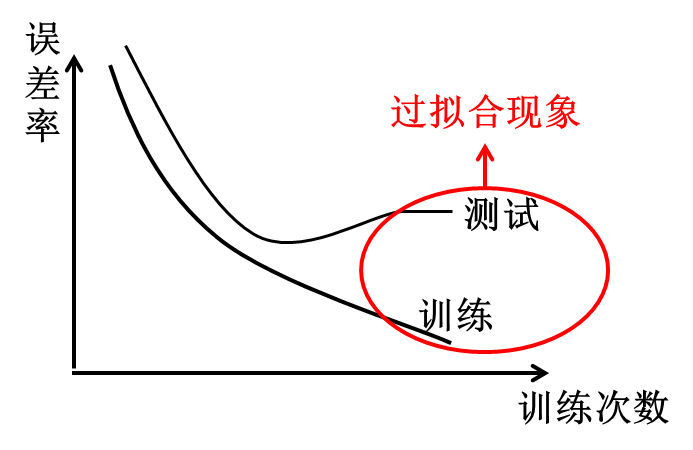
\includegraphics[height=4cm]{images/Adaboost1.jpg}
  				\end{varwidth}
  				\qquad
  				\begin{varwidth}[t]{\textwidth}
    			\vspace{0pt}
    			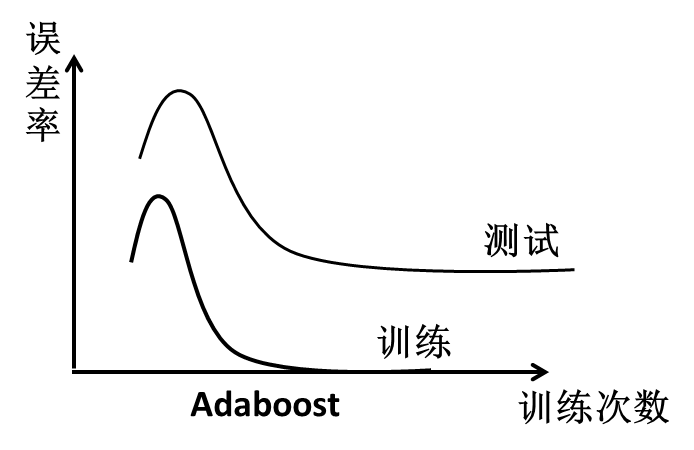
\includegraphics[height=4cm]{images/Adaboost2.jpg}
  				\end{varwidth}
				\caption{Adaboost误差率示意图}
				\label{fig:Adaboost误差率示意图}
				\end{figure}
            % \textcolor[rgb]{1 0 0}{todo:图片:Adaboost误差率示意图}\\
            并且从图(\ref{fig:Adaboost误差率示意图})右图可以看到,在训练误差达到0以后的一段时间内,AdaBoost的测试误差仍在下降,这是AdaBoost很“迷人”的地方。为了回答AdaBoost的泛化能力从何而来,AdaBoost的作者Schapire将统计学习中分类间隔分析的相关理论引入到AdaBoost的分析当中:
            \begin{definition}
            $F = \sum_i \alpha_i f_i(x)$的分类间隔为
            \begin{align*}
            margin_+ (x,y) = y\sum_i\alpha_i f_i(x)\big/\sum_i|\alpha_i| \quad \in [-1,1]
            \end{align*}
            分类间隔的符号为正,则表示分类正确,反之为错误分类,其取值反应了分类结果的可信程度。
            \end{definition}
            \begin{theorem}
            设$D$是定义在$X\times \{-1,1\}$上的分布函数,训练样本集$S$依分布$D$独立随机采样。若子分类器可行空间$f\in H$有限,$C = \{f:x\to \sum_{f\in H}\alpha_h f(x)|\alpha_h \geqslant 0,\sum_h \alpha_h=1\}$,对$\theta>0,\delta >0$,每一个$f\in C$以$1-\delta$的概率满足如下错误率限界\cite{1997.Schapire}
            \begin{align*}
            P_D(margin_+ (x,y) \leqslant0) \leqslant P_s(margin_+ (x,y) \leqslant\theta) + O \left( \frac{1}{\sqrt{m}} \left( \frac{\log m\log |H|}{\theta^2} +\log \frac{1}{\delta}\right)^\frac{1}{2}  \right)
            \end{align*}
            其中:$P_s$是训练集的分类间隔分布,$m$为样本数,子分类器$f$的可行空间大小是$|H|$(通常以VC维度量)。
            \end{theorem}
            \par
            注意,上面的定理给出的泛化误差界$P_D$是非常松弛的,并且不具有渐进性,只有当训练集中的样本数目很大时才有意义,而当样本量很小时,这一误差界并不准确。如何寻找一个更紧致的泛化误差界以指导算法的设计仍然是一个困难的工作。
            \par
            1996.Freund在\cite{1996.Freund}中提出了AdaBoost.M1和AdaBoost.M2两种算法。AdaBoost.M1即是我们常见的Discrate AdaBoost,而AdaBoost.M2是M1的泛化形式。该文的一个结论是:当弱分类器使用简单分类方法时,boosting的效果统一比bagging要好;当弱分类器使用C4.5时,boosting比bagging要好。1998.Schapire R E和Singer Y\cite{1998.Schapire}提出更具一般性的AdaBoost形式,提出自信率以改善AdaBoost的性能,并提出了解决多分类问题的AdaBoost.MH(Real Boost)和AdaBoost.MR。事实上,Discrete到Real的转变体现了古典集合到模糊集合的转变。


      \subsection{加法模型}
          \par
          Friedman\cite{2000.Friedman}等从统计学角度出发,在非参数回归的基础上,给出了加法模型的前向顺序算法。尽管这样解释受到了质疑,被认为不能有效解释AdaBoost的泛化能力,但在此理论基础上衍生出了许多重要的AdaBoost算法,后面要介绍的GBDT就是其中一种,此外还有LogitBoost、fradient-boost-tree以及用于解决概率回归的ProbitBoost。
          \par
          考虑二分类问题,并设置$y^k\in \{-1,1\}$。上面我们一共有$M$个弱分类器,并且最终的分类器(强分类器)是$M$个弱分类器的组合。现在,我们将最终的强分类器写为\cite{2009.Rojas}
          \begin{align*}
          F_M(x) = \frac{1}{2}\sum_{i=1}^M\alpha_i f_i(x)
          \end{align*}
          上式可以表示为
          \begin{align*}
          F_M(x) = F_{M-1}(x)+\frac{1}{2}\alpha_Mf_M(x)
          \end{align*}
          这里将$F_M(x)$作为直接的分类器,建立整体分类模型,设置模型的损失函数为
          \begin{align*}
          E = \sum_{k=1}^me^{-y^kF_M(x^k)}
          \end{align*}
          当$F_M(x^k) = y^k$时,$e^{-y^kF_M(x^k)} = e^{-1}$;当$F_M(x^k) =- y^k$时,$e^{-y^kF_M(x^k)} = e^{1}$。
          \par
          我们的目标是求参数$\alpha = (\alpha_1,\alpha_2,\dots,\alpha_M)$以及$f_i(x)$中的参数$\theta$,使$E$最小。这是一个非常复杂的优化问题,并不易于求解(这个地方好像与神经网络有关,以后再看)。下面,介绍前向分步算法:每次只求一个$\alpha_i,f_i(x)$,其余$\alpha_{-i},f_{-i}(x)$保持不变。由此,可以将$E$进行拆分:固定一组,待求一组。不失为一般性,我们假设求$\alpha_M,f_M$,于是$E$拆分为
          \begin{align*}
          E & = \sum_{k=1}^m\exp\left\{-y^k\left[F_{M-1}(x^k)+ \frac{1}{2}\alpha_M f_M(x^k)\right]\right\}\\
          & = \sum_{k=1}^m \exp\left\{-y^kF_{M-1}(x^k)-\frac{1}{2}y^k\alpha_M f_M(x^k)   \right\}\\
          &= \sum_{k=1}^m w_M^k \exp\left\{ -\frac{1}{2}y^k\alpha_Mf_M(x^k) \right\}
          \end{align*}
          其中:$w_M^k = \exp \{-y^k F_{M-1}(x^k)\}$,且$\sum w_M^k=1$,$M>1$。
          \par
          求最值,要将$E$对$\alpha_M$和$f_M$求导。在此之前,将被$f_M(x)$正确分类的样本集合记为$T_M$,剩下误分类样本记为$M_M$,于是可以将上式拆分为
          \begin{align}
          \label{加法模型的目标函数}
          E & = e^{-\frac{\alpha_M}{2}} \sum_{k\in T_M}w_M^k + e^{\frac{\alpha_M}{2}} \sum_{k\in M_M}w_M^k \\
          & = e^{-\frac{\alpha_M}{2}}\sum_{k=1}^m w_M^k + \left( e^{\frac{\alpha_M}{2}} - e^{-\frac{\alpha_M}{2}} \right)  \sum_{k=1}^mw_M^k I_{f_M(x^k) \neq y^k} \notag
          \end{align}
          其中:$f_M(x^k)$是第$M$个分类器对第$k$个样本$x^k$的分类结果,$y^k$为第$k$个样本的真实类别。现在,我们再将$E$对$\alpha_M$和$f_M$求导:
          \par
          (1)关于$f_M$的求导。注意到$w_M^k$是常量,因此
          \begin{align*}
          \frac{\partial E}{\partial f_M(\theta)} = \left( e^{\frac{\alpha_M}{2}} - e^{-\frac{\alpha_M}{2}} \right) \frac{\partial }{\partial f_M(\theta)}\sum_{k=1}^m I_{f_M(x^k)\neq y^k}
          \end{align*}
          上式与单一模型$J_M = \sum_{k=1}^m w_M^k I_{f_M(x^k)\neq y^k} $(这是第$M$个模型)关于$f$求导是等价的。
          \par
          (2)关于$\alpha_M$求导。注意,这里用(\ref{加法模型的目标函数})式比较方便,有
          \begin{align*}
          \frac{\partial E}{\partial \alpha_M} = -\frac{1}{2}e^{-\frac{\alpha_M}{2}}\sum_{k\in T_M}w_M^k + \frac{1}{2} e^{\frac{\alpha_M}{2}}\sum_{k\in M_M}w_M^k
          \end{align*}
          令上式等于0,有
          \begin{align*}
          \alpha_M = \ln \left( \frac{\sum\limits_{k\in T_M}w_M^k}{\sum\limits_{k\in M_M}w_M^k} \right)
          \end{align*}
          我们令
          \begin{align*}
          \epsilon_M = \frac{\sum\limits_{k\in M_M}w_M^k }{\sum\limits_{k=1}^m w_M^k} = \frac{\sum\limits_{k=1}^mw_M^kI_{f_M(x^k)\neq y^k}}{\sum\limits_{k=1}^m w_M^k} = \frac{1-\sum\limits_{k\in T_M} w_M^k}{\sum\limits_{k=1}^m w_M^k}
          \end{align*}
          上式用到了
          \begin{align*}
          \sum_{k=1}^m w_M^k = \sum_{k\in T_M} + \sum_{k\in M_M}
          \end{align*}
          将$\epsilon_M$带入到$\alpha_M$,我们有
          \begin{align*}
          \alpha_M= \ln \left( \frac{1-\epsilon_M}{\epsilon_M} \right)
          \end{align*}
          \par
          上面给出了$E$对$\alpha_M$和$f_M$求导。根据$E$的计算公式(\ref{加法模型的目标函数}),我们看到,在解出$\alpha_M$和$f_M(x)$之后,样本权重由下式更新
          \begin{align*}
          w_{M+1}^k = w_M^k \exp\left\{-\frac{1}{2} y^k \alpha_M f_M(x^k)  \right\}
          \end{align*}
          由于
          \begin{align*}
          y^k f_M(x^k) = 1-2 I_{f_M(x^k)\neq y^k}
          \end{align*}
          我们有
          \begin{align*}
          w_{M+1}^k = w_M^k\exp \left(- \frac{\alpha_M}{2} \right) \exp\left\{\alpha_M I_{f_M(x^k) \neq y^k}\right\}
          \end{align*}
          由于$\exp (- \frac{\alpha_M}{2} )$与$k$无关,对所有样本都有一个这样的因子,因此,我们可以将其忽略。这样,我们就得到了样本权重的更新公式。
          \par
          此外,对于$\alpha_M$的选取,我们还有如下结论。我们选择$\alpha_M$使指数误差函数最小,简写为
          \begin{align*}
          E = \sum_k w^k e^{-y^k f_M(x^k)\alpha_M}
          \end{align*}
          假设$f_M(x^k)$已有,记为$f^k$,且$y^k\in \{-1,1\}$,则
          \begin{align*}
          E = \sum_k w^k e^{-y^k f^k \alpha_M}
          \end{align*}
          我们有
          \begin{align*}
          \sum_k w^k e^{-y^k f^k \alpha_M} & \leqslant \sum_k \left( \frac{1-y^k f^k}{2} \right)w^k e^{\alpha_M} + \sum_k \left( \frac{1+y^k f^k}{2} \right) w^k e^{-\alpha_M} \\
          & = \left( \frac{1+\epsilon_M}{2} \right) e^{\alpha_M} + \left( \frac{1-\epsilon_M}{2} \right) e^{-\alpha_M}
          \end{align*}
          令上式等于0,我们可以找到最小的上界
          \begin{align*}
          \alpha_M' = \frac{1}{2}\ln \left( \frac{1-\epsilon_M}{1+\epsilon_M} \right)
          \end{align*}
          \par
          注意:这里只适用二分类情况$y^k\in \{-1,1\}$,但是它可以推广到多分类以及回归问题。上面,我们将boosting方法转换成可加模型的指数误差优化模型,如果我们使用不同的目标函数,这种转换可以引出一大类与Adaboost相似的算法。我们称这种多模型相加的模型为可加模型,称这种逐步一次计算一个模型及参数的优化方法为前向分步算法或前向顺序算法。

      \subsection{GBDT}
          \par
          根据上面的加法模型,如果设置不同的弱分类器$f$和不同的损失函数,我们可以得到许多不同的boost方法。我们以决策树作为弱分类器,构建的加法模型为提升树模型(boost tree)。将整体分类函数记为
          \begin{align*}
          F_M(x) = \sum_{i=1}^M f(x;\theta_i)
          \end{align*}
          其中:$f(x;\theta_i)$是第$i$个决策树,共有$M$个,$\theta_i$为决策树参数。我们可以将$F_M$进行拆分
          \begin{align*}
          F_M(x) = F_{M-1}(x)+f(x;\theta_M)
          \end{align*}
          我们通过经验风险最小化来确定决策树参数$\theta_M$
          \begin{align*}
          \hat{\theta}_M = \arg\min_{\theta_M}\ \sum_{k=1}^m L(y^k,F_M(x^k))
          \end{align*}
          其中:$L$为损失函数。在加法模型中,我们使用的是指数损失函数,选用不同的损失函数,可以得到不同的提升树。对于回归问题,我们可以采用$\frac{1}{2}(y^k-F_M(x^k))^2$或者$|y^k -F_M(x^k)|$作为损失函数;对于分类问题,我们使用指数损失,当然,我们还可以选择更一般的损失函数。关于损失函数的种类,我们在前面的神经网络部分有详细的介绍。
          \par
          加法模型中,我们使用指数损失处理了二分类问题,现在,我们来处理回归问题。在前向模型中,给定当前模型$F_{i-1}(x)$,需要求解
          \begin{align*}
          \hat{\theta}_i = \arg\min_{\theta_i} \ \sum_{k=1}^m L(y^k,f(x^k;\theta_i))
          \end{align*}
          我们使用离差平方和作为损失函数
          \begin{align*}
          L(y^k,f(x^k)) = (y^k-f(x^k))^2
          \end{align*}
          于是有
          \begin{align*}
          \min_{\theta_i}\ J(\theta_i) & = \sum_{k=1}^m (y^k - F_{i-1}(x^k) -f(x^k;\theta_i))^2\\
          & = \sum_{k=1}^m (r_{i-1}^k - f(x^k;\theta_i))^2
          \end{align*}
          其中:$r_{i-1}^k = y^k - F_{i-1}(x^k)$为第$i-1$次的误差。也就是说,上述过程是用第$i$个模型$f_i$来拟合模型的第$i-1$次的残差$r_{i-1}$。所以,对回归问题而言,AdaBoost只需要简单得拟合前模型$F_{i-1}$的误差$r_{i-1}$即可。
          \par
          上面仍然是在介绍加法模型,下面来具体的介绍GBDT(梯度提升模型)。在上面的加法模型中,当损失函数$L$是平方损失或者指数损失时,每一步优化是简单的,但对于一般的损失函数$L$而言则不是易于处理的,比如绝对损失和Huber损失等。为此,Freidman提出Gradient Boosting\cite{2000.Frie},GBDT的核心在于:每一个子分类器$f_i(x) \triangleq f(x;\theta_i)$学习的是之前所有分类器的累加之和的残差。每一次迭代减少上一模型的残差,并且在残差减少的梯度方向上建立新的组合模型。在此之前,我们先来看一个引例。
          \par
          考虑一般的线性回归模型
          \begin{align*}
          \hat{y} = f(x;\theta_1) = w^\mathrm{T}x + b
          \end{align*}
          我们用$f$对$y$进行估计后,二者之间会有一个误差$\epsilon\in R^m$($m$个样本)。如果我们想要改进$f$,一个可行的方法是缩小它的残差,那么,我们可以对$y,f(x)$的残差进行估计,把估计的残差在加入到$f$中,即
          \begin{align*}
          \hat{y} = f+\hat{\varepsilon}
          \end{align*}
          为了便于处理,我们仍然用$f$对$\varepsilon$进行估计
          \begin{align*}
          \hat{\varepsilon} = f(x;\theta_2)
          \end{align*}
          于是有
          \begin{align*}
          \hat{y} = f(x;\theta_1)+f(x;\theta_2)
          \end{align*}
          用上式对$y$进行估计后,必然会有新的残差,我们仍然对新的残差进行估计,然后把估计的残差加入到上一个模型当中,如此反复下去
          \begin{align*}
          & \hat{y} = f_1\\
          & \hat{y} = f_1+f_2\\
          & \quad \vdots\\
          & \hat{y} = f_1+f_2+\cdot+f_M
          \end{align*}
          \par
          将上述方法规范化,写成加法模型的形式
          \begin{align*}
          & F_i(x) =F_{i-1}(x)+\alpha_if_i(x;\theta_i)\\
          & F_M = \sum_{i=1}^M \alpha_i f_i(x)
          \end{align*}
          并设置目标
          \begin{align*}
          \{\theta_i,\alpha_i\}_{i=1}^M = \arg\min_{\theta,\alpha} \ J(\theta,\alpha) = \sum_{k=1}^m L(y^k,F_M(x^k))
          \end{align*}
          上述优化问题较复杂,我们采用前面介绍的分步前向算法,有
          \begin{align*}
          (\theta_i,\alpha_i) = \arg\min \ \sum_{k=1}^m L(y^k,F_{i-1}(x^k)+\alpha_i f_i(x^k;\theta_i))
          \end{align*}
          现在的问题是,如何求解新加入的$f_i$和$\alpha_i$?可以观察到$F_i(x) =F_{i-1}(x)+\alpha_if_i(x;\theta_i)$和优化模型中的更新方程$x_{i} = x_{i-1}+\alpha_i \Delta x_i$很相似,如果将$f_i(x;\theta_i)$视为$\Delta F_i(x)$,则有
          \begin{align*}
          F_i = F_{i-1}+\alpha_i \Delta F_i
          \end{align*}
          那么,我们能否将$f_i$视为目标$J$的梯度方向呢?我们在函数空间上\underline{形式的}对$F$求导,有
          \begin{align*}
          g_i(x) = -\frac{\partial E[L(y,F(x))]}{\partial F(x)} \bigg|_{F(x) = F_{i-1}(x)}
          \end{align*}
          $g_i(x)$即为$F$的负梯度方向(这里的$g_i$就等价于前面的残差$r_i$)。为了更新$F$,接下来我们只要求出步长$\alpha_i$即可
          \begin{align*}
          \alpha_i = \arg\min_\alpha \ \sum_{k=1}^m L(y^k,F_{i-1}(x^k)+\alpha f_i(x^k;\theta_i))
          \end{align*}
          于是有下面的算法(\ref{code:GBDT})
          \begin{algorithm}[H]
              \caption{GBDT}\label{code:GBDT}
              \begin{algorithmic}[1]
                  \State $F_0(x) = f_0(x)$。
                  \For {$i = 1,2,\dots,M$}
                      \State $//$计算梯度$g_i$
                      \For {$k=1,2,\dots,m$}
                          \State $g_i(x^k) = -\frac{\partial E[L(y,F(x^k))]}{\partial F(x^k)} \Big|_{F(x^k) = F_{m-1}(x^k)}$
                      \EndFor
                      \State 计算步长$\alpha_i$。$\alpha_i = \arg\min \ E[L(y,F_{i-1}(x)+\alpha_i g_i(x))]$
                      \State 计算更新量。$f_i(x) = \alpha_i g_i(x)$
                      \State 更新函数。$F_i(x) = F_{i-1}(x)+f_i(x) = F_{i-1}(x) +\alpha_i g_i(x)$
                  \EndFor
                  \State 输出。$F= F_M(x) = f_0 + \sum_{i=1}^M \alpha_i f_i(x)$
              \end{algorithmic}
          \end{algorithm}
          \par
          上面介绍了一般形式的GBDT算法,下面,我们给出一些损失函数$L$下的GBDT算法。
          \subsubsection{L$\_$2 - TreeBoost}
              \par
              考虑二分类问题$y^k\in \{-1,1\}$,使用决策树作为子分类器,使用negative binomial log-likelihood作为损失函数(在加法模型中,我们使用了指数损失),log损失函数定义为
              \begin{align*}
              L(y,F) = \log (1+e^{-2yF})
              \end{align*}
              现在,我们用上面介绍的GBDT算法来求解上述问题:\\
              \textbf{Step1.}求第一个分类器
              \begin{align*}
              F_0 = f_0 = \arg\min\ J(F) = \sum_{k=1}^m L(y^k,F)
              \end{align*}
              $J(F)$关于$F$求导,有
              \begin{align*}
              &\frac{\partial }{\partial F} \sum_{k=1}^m L(y^k,F)\\
              ={} &\sum_{k=1}^m \frac{e^{-2y^k F} -2y^k}{1+e^{-2y^k F}}\\
              ={} &\sum_{k:y^k=1}\frac{-2e^{2F}}{1+e^{-2F}}+ \sum_{k:y^k = -1}\frac{2e^{2F}}{1+e^{2F}}
              \end{align*}
              令上式为0,有
              \begin{align*}
              F_0(x) = \frac{1}{2}\log \frac{1+\bar{y}}{1-\bar{y}}
              \end{align*}
              \textbf{Step2.}对$g_i(x)$进行求解
              \begin{align*}
              g_i(x^k) =& -\frac{\partial L(y^k,F)}{\partial F}\bigg|_{F = F_{i-1}}\\
              =& \frac{-2y^k e^{-2y^k F}}{1+e^{-2y^kF}}\bigg|_{F = F_{i-1}}\\
              =& \frac{-2y^k e^{-2y^k F_{i-1}(x^k)}}{1+e^{-2y^k F_{i-1}(x^k)}}\\
              =& \frac{2y^k}{1+e^{2y^k F_{i-1}(x^k)}}
              \end{align*}
              \textbf{Step3.}用决策树$f_i$对$g_i(x)$进行估计,求解$\theta_i$。\\
              \textbf{Step4.}用一个牛顿法求步长$\alpha_i$
              \begin{align*}
              \alpha_i = \arg\min_\alpha\ \sum_{k=1}^m \log (1+\exp\{-2y^k(F_{i-1}(x^k)+\alpha f(x^k;\theta_i))\})
              \end{align*}
              我们仍然使用决策树作为基本分类器,仍然要划分一个根节点
              \begin{align*}
              \alpha_{li} = \arg\min_\alpha \ \sum_{x^k\in R_{li}}\log (1+\exp\{-2y^k(F_{i-1}(x^k)+\alpha f_{li})\})
              \end{align*}
              或者
              \begin{align}
              \label{L2TreeBoost的步长}
              & r_{li} = \alpha_{li}h_{li} = \arg\min_r \ \sum_{x^k\in R_{li}} \log (1+\exp\{-2y^k(F_{i-1}(x^k)+r)\})\\
              & F_i(x) = F_{i-1}(x)+r_{li}I({x\in R_{li}}) \notag
              \end{align}
              我们可以使用a single Newton-Raphson step来求式(\ref{L2TreeBoost的步长})
              \begin{align*}
              r_{li} = \frac{\sum\limits_{x^k\in R_{li}} g^k}{\sum\limits_{x^k\in R_{li}}|g^k|(2-|g^k|)}
              \end{align*}
              综上,有算法(\ref{code:L2-TreeBoost})
              \begin{algorithm}[H]
                  \caption{L2-TreeBoost}\label{code:L2-TreeBoost}
                  \begin{algorithmic}[1]
                      \State $F_0(x) = \frac{1}{2}\log \frac{1+\bar{y}}{1-\bar{y}}$。
                      \For {$i = 1,2,\dots,M$}
                          \State $//$计算梯度$g_i$
                          \For {$k=1,2,\dots,m$}
                              \State $g^k = -\frac{2y^k}{1+e^{2y^k F_{i-1}(x^k)}}$
                          \EndFor
                          \State $\{R_{li}\}_{l=1}^L = L\_terminal\_mode\_tree(\{x^k,g^k\}_{k=1}^m)$
                          \State $r_{li} = \frac{\sum\limits_{x^k\in R_{li}} g^k}{\sum\limits_{x^k\in R_{li}}|g^k|(2-|g^k|)}\quad l=1,2,\dots,L$
                          \State $F_i(x) = F_{i-1}(x)+r_{li}I({x\in R_{li}})$;
                      \EndFor
                  \end{algorithmic}
              \end{algorithm}
              \par
              设
              \begin{align*}
              p_+(x) = \hat{P}(y=1|x) = 1/(1+\exp\{-2F_M(x)\})\\
              p_-(x) = \hat{P}(y=-1|x) = 1/(1+\exp\{2F_M(x)\})
              \end{align*}
              则最终的分类估计为
              \begin{align*}
              \hat{y}(x) = 2I(c(-1,1)p_+>c(1,-1)p_-(x))-1
              \end{align*}
              其中:$c(\hat{y},y)$ is the cost associated with predicting $\hat{y}$ when the truth is $y$。例如$c(\hat{y},y) = 1$。
          \subsubsection{最小二乘损失:L2-Boost}
              \par
              设置损失函数为平方损失$L(y,F) = \frac{1}{2}(y-F)^2$,我们有算法(\ref{code:L2-Boost})
              \begin{algorithm}[H]
                  \caption{L2-Boost}\label{code:L2-Boost}
                  \begin{algorithmic}[1]
                      \State $F_0(x) = \bar{y}$。
                      \For {$i = 1,2,\dots,M$}
                          \State $//$计算梯度$g_i$
                          \For {$k=1,2,\dots,m$}
                              \State $g_i^k = y^k - F_{i-1}(x^k)$
                          \EndFor
                          \State 求参数$\theta_i$和步长$\alpha_i$。$(\theta_i,\alpha_i) = \arg\min_{\alpha,\theta} \ \sum_{k=1}^m [g^k - \alpha f(x^k;\theta)]^2$
                          \State $F_i(x) = F_{i-1}(x)+\alpha_i f_i(x;\theta_i)$;
                      \EndFor
                  \end{algorithmic}
              \end{algorithm}
          \subsubsection{绝对值损失:LAD-TreeBoost}
              \par
              设置损失函数为绝对值损失$L(y,F) = |y-F|$。\\
              (1)我们先来求解负梯度方向
              \begin{align*}
              g_i^k = g_i(x^k) & = -\left[\frac{\partial L(y^k,F(x^k))}{\partial F(x^k)}  \right]\bigg|_{F(x) = F_{i-1}(x^k)}\\
              & =sign[y^k - F_{i-1}(x^k)]
              \end{align*}
              (2)用$f_i$去拟合$g_i$,求得$\theta_i$,然后求步长$\alpha_i$
              \begin{align*}
              \alpha_i  &=\arg\min_\alpha \sum_{k=1}^m L(y^k ,F_{i-1}(x^k)+\alpha f(x^k;\theta_i))\\
              &=\arg\min_\alpha \sum_{k=1}^m |y_k - F_{i-1}(x^k)-\alpha f(x^k;\theta_i)|\\
              &=\arg\min_\alpha \sum_{k=1}^m |f(x^k;\theta_i| \cdot \left|\frac{y^k - F_{i-1}(x^k)}{f(x^k;\theta_i)}-\alpha \right|\\
              & = median_w\left\{ \frac{y^k - F_{i-1}(x^k)}{f(x^k;\theta_i)} \right\}_{k=1}^m,\quad w^k = |f(x^k;\theta_i)|
              \end{align*}
              其中:$median_w$是权重$w^i$的中值,$f_i(x^k,;\theta_i)$是一个$L$个末端节点的决策树。关于上面的计算,我们把参数$P = \{\alpha_i,\theta_i\}$分割成$L$个子集$P_1,P_2,\dots,P_L$,梯度是相对分段的。
              \begin{align}
              \label{绝对损失的权重公式}
              \alpha_{li} = median_w\left\{\frac{y^k - F_{i-1}(x^k)}{f(x^k;\theta_i)} \bigg|x^k \in R_{li}  \right\} \quad w^k = |f_i(x^k;\theta_i)|
              \end{align}
              $L$为决策树叶节点数,$R_{li}$是$x$的空间。由于$\{f(x^k;\theta_i)|x^k\in R_{li}\}$的值是全部相等的$f(x^k;\theta_i) = f_{li}I({x^k\in R_{li}})$,因此,对于式(\ref{绝对损失的权重公式})我们有
              \begin{align*}
              \alpha_{li} = \frac{1}{f_{li}}median\{y^k-F_{i-1}(x^k)|x^k\in R_{li}\}
              \end{align*}
              并且,GBDT的更新公式变为
              \begin{align*}
              F_i(x) = F_{i-1}(x)+median\{y^k-F_{i-1}(x^k)|x^k\in R_{li}\}I(x\in R_{li})
              \end{align*}
              \par
              上面给出了基于绝对误损失的梯度提升树,下面,我们给出LAD-TreeBoost算法的伪代码(\ref{code:LAD-TreeBoost})
              \begin{algorithm}[H]
                  \caption{LAD-TreeBoost}\label{code:LAD-TreeBoost}
                  \begin{algorithmic}[1]
                      \State $F_0(x) = median\{y^k\}_{k=1}^m$。
                      \For {$i = 1,2,\dots,M$}
                          \State 计算梯度$g^k = sign(y^k - F_{i-1}(x^k))$
                          \State $\{R_{li}\}_{l=1}^L = L\_terminal\_node\_tree(\{x^k,g^k\}_{k=1}^m)$
                          \State $r_{li} = median_{x\in R_{li}}(y^k - F_{i-1}(x^k)),l = 1,2,\dots,L$ 。
                          \State $F_i(x) = F_{i-1}(x) + r_{li}I(x\in R_{li})$
                      \EndFor
                  \end{algorithmic}
              \end{algorithm}
          \subsubsection{Huber损失}
              \par
              下面,我们将损失设定为Huber损失,该损失是Huber于1964年提出,其形式为
              \begin{align*}
              L(y,F) = \left\{
              \begin{aligned}
              \frac{1}{2}(y-F)^2\quad |y-F| \leqslant \delta\\
              \delta (|y-F|-\frac{\delta}{2}) \quad |y-F| > \delta
              \end{aligned}
              \right.
              \end{align*}
              \par
              (1)$L$关于$F$求导,有
              \begin{align*}
              g^k =& -\frac{\partial L(y^k,F(x^k))}{\partial F(x^k)} \bigg|_{F(x) = F_{i-1}(x^k)}\\
              =& \left\{
              \begin{aligned}
              & y^k - F_{i-1}(x^k) \quad |y-F| \leqslant \delta\\
              & \delta sign (y^k - F_{i-1}(x^k)) \quad |y-F| >\delta
              \end{aligned}
              \right.
              \end{align*}
              \par
              (2)步长$\alpha_i$为
              \begin{align*}
              \alpha_i = \arg\min_\alpha \ \sum_{k=1}^m L(y^k,F_{i-1}(x^k)+\alpha f(x^k;\theta_i))
              \end{align*}
              转折点$\delta$依赖于迭代次数$i$,详细的说,$\delta_i$是$\{|y^k - F{i-1}(x^k)|\}_{k=1}^m$的$\alpha$分位数。
              \par
              我们选用决策树作为基本分类器(子分类器),使用分割策略在每个$R_{li}$中查找$\alpha_i$
              \begin{align*}
              \alpha_{li} = \arg\min_\alpha \ \sum_{x^k\in R_{li}} L(y^k,F_{i-1}(x^k)+\alpha f_{li})
              \end{align*}
              最终的更新公式为
              \begin{align*}
              F_i(x) = F_{i-1}(x)+r_{li}I(x\in R_{li})
              \end{align*}
              其中:$r_{li} = \alpha_{li}f_{li} = \arg\min_r\sum_{x^k\in R_{li}}L(y^k,F_{i-1}(x^k)+r)  $。Huber1964年给出$r_{li}$的简单一步估计
              \begin{align*}
              \tilde{r}_{li} = median_{x^k\in R_{li}} \{r_{{i-1}}(x^k)\}
              \end{align*}
              这里$\{r_{i-1}\}_{i=1}^M$ are the current redsiduals $r_{l_{i-1}}(x^k) = y^k - F_{i-1}(x^k)$,最终$r_{li}$的近似为
              \begin{align*}
              r_{li} = \tilde{r}_{li} + \frac{1}{N_{li}} \sum_{x^k\in R_{li}}sign (r_{i-1}(x^k) - \tilde{r}_{li})\cdot \min(\delta_i,|r_{i-1}(x^k| - \tilde{r}_{li})
              \end{align*}
              其中:$N_{li}$是第$l$个节点的样本数。下面,给出Huber\ M-TreeBoost算法(\ref{code:Huber M-TreeBoost})
              \begin{algorithm}[H]
                  \caption{Huber M-TreeBoost}\label{code:Huber M-TreeBoost}
                  \begin{algorithmic}[1]
                      \State $F_0(x) = median\{y^k\}_{k=1}^m$。
                      \For {$i = 1,2,\dots,M$}
                          \State $r_{i-1}(x^k) = y^k - F_{i-1}(x^k),k=1,2,\dots,m$;
                          \State $\delta_i = quantile_\alpha\{|r_{i-1}(x^k)|\}_{k=1}^m$;
                          \State \[ g^k = \left\{
                          \begin{aligned}
                          r_{i-1}(x^k) \quad |r_{i-1}(x^k)| \leqslant \delta_i\\
                          \delta_isign(r_{i-1}(x^k))\quad |r_{i-1}(x^k)|>\delta_i
                          \end{aligned}
                          \right. \]
                          \State $\{R_{li}\}_{l=1}^L = L\_terminal\_node\_tree(\{x^k,g^k\}_{k=1}^m)$
                          \State $\tilde{r}_{li} = median_{x^k\in R_{li}} \{r_{{i-1}}(x^k)\} ,l=1,2,\dots,L$
                          \State $r_{li} = \tilde{r}_{li} + \frac{1}{N_{li}} \sum\limits_{x^k\in R_{li}}sign (r_{i-1}(x^k) - \tilde{r}_{li})\cdot \min(\delta_i,|r_{i-1}(x^k| - \tilde{r}_{li}),l = 1,2,\dots,L$ 。
                          \State $F_i(x) = F_{i-1}(x) + r_{li}I(x\in R_{li})$
                      \EndFor
                  \end{algorithmic}
              \end{algorithm}
          \subsubsection{多分类Boost}
              \par
              上面的GBDT都是处理二分类问题的,下面我们考虑一个$C$分类问题。定义损失函数为
              \begin{align*}
              L(\{y_c,F_c(x)\}_{c=1}^C) = -\sum_{c=1}^C y_c \log p_c(x)
              \end{align*}
              其中:$y_c = 1\in \{0,1\}$,$p_c(x) =  P(y_c = 1|x)$,we use the symmetric multiple logistic transform
              \begin{align*}
              F_c(x) = \log p_c(x) - \frac{1}{C}\sum_{c=1}^C\log p_c(x)
              \end{align*}
              or equivalently
              \begin{align*}
              p_c(x) = \frac{e^{F_c(x)}}{\sum_c e^{F_c(x)}}
              \end{align*}
              \par
              先来求梯度
              \begin{align*}
              g_c^k =&  -\frac{\partial L(\{y_c^k,F_c(x^k)\}_{c=1}^C)}{\partial F_c(x^k)} \bigg|_{\{F_c(x^k) = F_{c,i-1}(x^k)\}_1^C}\\
              =& y_c^k - p_c(x^k)
              \end{align*}
              对于残差$\{y_c^k - p_c(x^k)\}_{k=1}^m$,我们使用$C$个树,每个树有$L$个叶节点,将样本空间划分为$R_{cli}$
              \begin{align*}
              r_{cli} = \arg\min_r \sum_{x^k\in R_{cli}} \phi_c(y_c^k,F_{c,i-1}(x^k)+r)
              \end{align*}
              其中:$\phi_c = -y_c\log p_c(x)$。$C$个函数每一个的更新公式为
              \begin{align*}
              F_{c,i}(x) = F_{c,i-1}(x) + r_{cli}I(x\in R_{cli})
              \end{align*}
              我们仍然用一个a single Newton-Raphson来逼近$r_{cli}$,有
              \begin{align*}
              r_{cli} = \frac{C-1}{C} \frac{\sum_{x^k\in R_{cli}}g_c^k}{\sum_{x^k\in R_{cli}}|g_{c}^k|(1-|g_c^k|)}
              \end{align*}
              综上,我们有算法(\ref{code:Lk-TreeBoost})
              \begin{algorithm}[H]
                  \caption{Lk-TreeBoost}\label{code:Lk-TreeBoost}
                  \begin{algorithmic}[1]
                      \State $F_{c0}(x) = 0,c = 1,2,\dots,C$。
                      \For {$i = 1,2,\dots,M$}
                          \State $p_c(x) = \frac{e^{F_c(x)}}{\sum_c e^{F_c(x)}},c=1,2,\dots,c$;
                          \For {$c = 1,2,\dots,C$}
                              \State $g_c^k = y_c^k - p_c(x^k),k=1,2,\dots,m$;
                              \State $\{R_{cli}\}_{l=1}^L = L\_terminal\_node\_tree(\{x^k,g_c^k\}_{k=1}^m)$
                              \State $r_{cli} = \frac{C-1}{C} \frac{\sum_{x^k\in R_{cli}}g_c^k}{\sum_{x^k\in R_{cli}}|g_{c}^k|(1-|g_c^k|)},l=1,2,\dots,L$ ;
                              \State $F_{c,i}(x) = F_{c,i-1}(x) + r_{cli}I(x\in R_{cli})$
                          \EndFor
                      \EndFor
                      \State 输出$\{F_{c,M}(x)\}_{c=1}^C$
                  \end{algorithmic}
              \end{algorithm}
              \par
              $\{F_{c,M}(x)\}_{c=1}^C$即是最终的分类器,通过$\{F_{c,M}(x)\}_{c=1}^C$我们可以获得$\{p_{c,M}(x)\}_{c=1}^C$的一致估计量
              \begin{align*}
              \hat{C}(x) = \arg\min_{1 \leqslant c \leqslant C}\sum_{c'=1}^C \mathrm{cost}(c,c')p_{c',M}(x)
              \end{align*}
              其中:$\mathrm{cost}(c,c')$ is the cost associated with predicting the $c$th class with the truth is $c'$.
              \par
              注:1. GBDT是串行运行的,并不适用于并行处理,因为当前时刻的迭代与上一时刻迭代结果有关。关于GBDT的并行处理,以后再详细讨论;2.对于加法模型而言,我们将其视为一个整体分类/回归模型,那么前面介绍的许多回归模型的改进方法(例如:正则化方法)都可以应用到加法模型上。

      \subsection{XGboost}
          \par
          仍然继续考虑前面的加法模型
          \begin{align*}
          & F_M(x) = \sum_{i=1}^M\alpha_i f_i(x;\theta_i)\\
          & F_i(x) = F_{i-1}(x)+\alpha_i f_i(x;\theta_i)
          \end{align*}
          我们设置加法模型的损失函数$L$以及优化的目标函数
          \begin{align*}
          \min\ J(\theta,\alpha) = \sum_{k=1}^m L(y^k,F_M(x^k))
          \end{align*}
          像前面的回归模型那样,我们对上述目标加上正则项$\Omega(f)$,有
          \begin{align*}
          \min \ \sum_{k=1}^m L(y^k,F_M(x^k))+\sum_{i=1}^M\Omega(f_i)
          \end{align*}
          假设基本分类器$f_i$是决策树,我们不能用SGD等方法来寻找$f$,因为$f$是决策树而不是数值向量(参数)。仍然采用加法模型中的分步前向算法来求解单一的树$f_i$及$\alpha_i$(求解$f_i$时,$f_j,j=1,2,\dots,l-1$是已知的),于是第$i$轮的目标为
          \begin{align*}
          (\theta_i,\alpha_i) & = \arg\min_{\alpha,\theta} \ \sum_{k=1}^m L(y^k,F_i(x^k)) + \sum_{j=1}^i \Omega(f_j)\\
          & = \arg\min_{\theta,\alpha}\ \sum_{k=1}^m L(y^k,F_{i-1}(x^k)+\alpha f_i(x^k;\theta)) +\sum_{j=1}^{i-1}\Omega(f_j)+\Omega(f_i)\\
          & = \arg\min_{\alpha,\theta} \ \sum_{k=1}^m L(y^k,F_{i-1}(x^k)+\alpha f_i(x^k;\theta))+\Omega(f_i)+constant
          \end{align*}
          设置损失函数是离差平方$L(y,F) = (y-F)^2$,于是有
          \begin{align}
          \label{XGboost目标}
          J(\theta,\alpha) & = \sum_{k=1}^m L(y^k,F_{i-1}(x^k)+\alpha f_i(x^k;\theta))+\Omega(f_i)+constant\\
          & = \sum_{k=1}^m (y^k - F_{i-1}(x^k)- \alpha f_i(x^k;\theta))^2 +\Omega (f_i)+constant\notag \\
          &= \sum_{k=1}^m([y^k-F_{i-1}(x^k)] - \alpha f_i(x^k;\theta))^2+\Omega(f_i)+constant\notag
          \end{align}
          现在,对$L$运用如下的泰勒展开公式
          \begin{align}
          \label{XGboost的泰勒公式}
          f(x+\Delta x) \approx f(x)+f'(x)\Delta x + \frac{1}{2}f''(x){\Delta x}^2
          \end{align}
          上述的$\Delta x$相当于我们的$f_i(x^k;\theta)$、$x$相当于$F$、$f$相当于目标$L$。定义
          \begin{align*}
          & g^k = \frac{\partial L(y^k,F(x^k))}{\partial F(x^k)}\bigg|_{F(x) = F_{i-1}(x)}\\
          & h^k = \frac{\partial^2 L(y^k,F(x^k))}{\partial F(x^k)^2}\bigg|_{F(x) = F_{i-1}(x)}
          \end{align*}
          则$L$的泰勒展开为
          \begin{align*}
           L(x^k,F_{i-1}(x^k)+\alpha f_i(x^k;\theta))
          \approx  L(y^k,F_{i}(x^k)) + g^k\alpha f_i(x^k;\theta)+\frac{1}{2}h^k (\alpha f_i(x^k;\theta))^2
          \end{align*}
          这里,$L$相当于泰勒公式(\ref{XGboost的泰勒公式})中的$f$、$F_{i-1}(x^k)$相当于$x$、$g^k$相当于$\Delta x$、$h^k$相当于$\Delta x^2$。式(\ref{XGboost目标})的目标$J$变为
          \begin{align}
          \label{XGboost目标2}
          J(\theta,\alpha) &= \sum_{k=1}^m L(y^k,F_{i-1}(x^k)+\alpha f_i(x^k;\theta))+\Omega(f_i)+constant\notag \\
          &\approx \sum_{k=1}^m \left[ L(y^k,F_{i}(x^k)) + g^k\alpha f_i(x^k;\theta)+\frac{1}{2}h^k (\alpha f_i(x^k;\theta))^2 \right]+ \Omega(f_i)+constant
          \end{align}
          \par
          如果对上面$L$的展开不是很清楚,可以看下面这个例子。考虑平方损失$L$的泰勒展开,$L$对于$F$\underline{形式上}的一阶导数为
          \begin{align*}
          g^k &= \frac{\partial L(y^k, F(x^k))}{\partial F(X^K)}\bigg|_{F(x) = F_{i-1}(x)}\\
          & = \frac{\partial (y^k - F(x^k))^2}{\partial F(x^k)}\bigg|_{F(x) = F_{i-1}(x)}\\
          & = 2(y^k - F(x^k))
          \end{align*}
          $L$对于$F$\underline{形式上}的二阶导数为
          \begin{align*}
          h^k & = \frac{\partial^2 L(y^k,F(x^k))}{\partial F(x^k)^2}\bigg|_{F(x) = F_{i-1}(x)}\\
          & = \frac{\partial ^2 (y^k - F(x^k))^2}{\partial F(x^k)^2}\bigg|_{F(x) = F_{i-1}(x)}\\
          & = \frac{\partial 2(y^k - F(x^k))}{\partial F(x^k)}\bigg|_{F(x) = F_{i-1}(x)}\\
          &=2
          \end{align*}
          \par
          注意到式(\ref{XGboost目标2})的$L(y^k,F_{i-1}(x^k))$是常量,可以移到constant中。于是,对$L$进行泰勒展开后,我们的目标是求$\alpha_i,f_i$(或者写为$\alpha_i,\theta_i$)使得下面的目标最小
          \begin{align}
          \label{XGboost目标3}
          J(\theta,\alpha) = \sum_{k=1}^m \left[g^k\alpha f_i(x^k;\theta)+\frac{1}{2}h^k(\alpha f_i(x^k;\theta))^2 \right]+\Omega(f_i)
          \end{align}
          上述目标是由式(\ref{XGboost目标2})去掉constant得到的,最优解$\alpha^*,\theta^*$即为$\alpha_i,\theta_i$。
          \par
          上面的GBDT是基于梯度的boost方法,而这里的XGboost是基于二阶导数的,我们称之为NewtonBoost。给出Newton Boost的一般算法框架(\ref{code:Newton Boost})
              \begin{algorithm}[H]
                  \caption{Newton Boost}\label{code:Newton Boost}
                  \begin{algorithmic}[1]
                      \State $F_0(x) = f_0(x) = \arg\min_\theta \sum_{k=1}^m L(y^k,f_0(x^k))$。
                      \For {$i = 1,2,\dots,M$}
                          \State $g_i^k =\frac{\partial L(y^k, F(x^k))}{\partial F(X^K)}\Big|_{F(x) = F_{i-1}(x)} ,k=1,2,\dots,m$;
                          \State $h_i^k =\frac{\partial^2 L(y^k, F(x^k))}{\partial F(X^K)^2}\Big|_{F(x) = F_{i-1}(x)} ,k=1,2,\dots,m$;
                          \State $\theta_i,\alpha_i = \arg\min\limits_{\theta,\alpha}\sum\limits_{k=1}^m \left[g^k\alpha f_i(x^k;\theta)+\frac{1}{2}h^k(\alpha f_i(x^k;\theta))^2 \right]+\Omega(f_i)$
                          \State $F_i(x) = F_{i-1}(x) + \alpha_if_i(x)$;
                      \EndFor
                  \end{algorithmic}
              \end{algorithm}
          \par
          下面,来考虑一个实际的决策树$f_i(x)$
          \begin{align*}
          f_i(x) = w_{q(x)}
          \end{align*}
          或者写为
          \begin{align*}
          f_i(x) = \sum_{j=1}^L w_j I(x\in R_j)
          \end{align*}
          其中:$f_i(x)$是含有$L$个叶节点的决策树, $q(x):R^n \to \{1,2,\dots,L\}$,$q(x^k)$将样本$x^k$投入到$L$个叶节点当中,$w\in R^L$是$L$个叶节点的权重。定义树$f_i$的正则项为
          \begin{align*}
          \Omega(f_i) = \gamma L+\frac{1}{2}\lambda \sum_{j=1}^L w_j^2
          \end{align*}
          其中:$\gamma L$表示惩罚树$f_i$的叶节点数量,$w_j$表示权重的惩罚。
          \par
          记样本集$S$中被投放到$j(j\in \{1,2,\dots,L\})$的子样本集$R_j = \{k|q(x^k) = j\},j = 1,2,\dots,L$,于是目标(\ref{XGboost目标3})可以具体写为
          \begin{align}
          \label{XGboost目标4}
          J(\theta,\alpha) =& \sum_{k=1}^m \left[ g^k \alpha w_{q(x^k)} + \frac{1}{2} h^k\alpha^2w^2_{q(x^k)} \right] + \gamma L + \frac{1}{2}\lambda \sum_{j=1}^L w_j^2 \notag \\
          =&\sum_{j=1}^L \left[ \left( \sum_{k\in R_j}g^k \right) \alpha w_j+\frac{1}{2} \left( \sum_{k\in R_j}(h^k\alpha^2 +\lambda)w_j^2 \right)   \right]+\gamma L
          \end{align}
          上面试和$L$独立的二次函数,我们先忽略$\alpha$,令$G_j = \sum_{k\in R_j}g^k$,$H_j = \sum_{k\in R_j}h^k$,则上述目标(\ref{XGboost目标4})写为
          \begin{align*}
          J(w,\gamma) =&  \sum_{j=1}^L \left[ \left( \sum_{k\in R_j}g^k \right)  w_j+\frac{1}{2} \left( \sum_{k\in R_j}(h^k +\lambda)w_j^2 \right)   \right]+\gamma L\\
          =& \sum_{j=1}^L \left[G_jw_j +\frac{1}{2}(H_j+\lambda)w_j^2\right]+\gamma L
          \end{align*}
          假设树$f_i$的结构$q(x)$是固定的,那么最优叶节点权重$w$及最优值为
          \begin{align*}
          & w_j^* = - \frac{G_j}{H_j+\lambda}\\
          & J^* = -\frac{1}{2} \sum_{j=1}^L \frac{G_j^2}{H_j+\lambda}+\gamma L
          \end{align*}
          注:对于$f = Gx + \frac{1}{2}Hx^2,H>0$,最小$x$在$x = -\frac{G}{H}$处获得,获得最小值为$f = -\frac{1}{2}\frac{G^2}{H}$。
          \par
          下面我们给出单一树的生成。\\
          \textbf{Step1.}列出可能的树的结构$q(x)$;\\
          \textbf{Step2.}计算$q(x)$的划分
          \begin{align*}
          J(x) = -\frac{1}{2}\sum_{j=1}^L \frac{G_j^2}{H_j+\alpha} + \gamma L
          \end{align*}
          \textbf{Step3.}找到最好的树的结构,并使用最优的权重
          \begin{align*}
          w_j^* = -\frac{G_j}{H_j+\lambda}
          \end{align*}
          \par
          不断地枚举不同树的结构,利用上式来寻找出一个最优结构的树,加入到模型中,再重复这样的操作。但是,这种可能的树的结构$q(x)$会有无穷多个,为此,我们使用Greedy learning来生成树,每一次尝试去对已有的叶子加入一个分割。对于一个具体的分割方案,我们可以获得的增益可以由如下方法计算
          :\\
          \textbf{Step1.}设置树的初始深度为0;\\
          \textbf{Step2.}对树的每个叶子节点尝试添加一个分割(split)节点,添加分割节点后的目标改变量为
          \begin{align*}
          Gain = \frac{G_L^2}{H_L+\lambda}+\frac{G_R^2}{H_R+\lambda} -\frac{(G_L+G_R)^2}{H_L+H_R+\lambda} - \gamma
          \end{align*}
          其中:$\frac{G_L^2}{H_L+\lambda}$是分割的左端的得分,$\frac{G_R^2}{H_R+\lambda}$是分割的右端的得分,$\frac{(G_L+G_R)^2}{H_L+H_R+\lambda}$是不分割的得分,$\gamma$是添加节点分割带来的复杂度。
          \par
          对于XGboost更详细的介绍可以参考\cite{2016.Tianqi}\cite{2016.Didrik}。文\cite{Wang.2016}分析了XGboost的代码及应用。下面简单介绍两个集成学习的“重器”——XGboost和LightGBM。
          % 文\cite{2016.Thomas}给出了XGboost、FastBDT、scikit-learn、TMVA之间的比较,
          \par
          注:如果不将GBDT和XGboost中的函数$f$设置为具体的分类器(比如$f$为决策树),也许可以在泛函问题上进行讨论。
        \subsection{应用示例-XGboost}
            \par
            XGboost\footnote{http://xgboost.readthedocs.io/en/latest/}是Tianqi Chen开发的C++的集成学习工具,并提供了Python、R和Scala等的API。XGboost的安装可以在网上查找,XGboost在Python下的参数解释可以参考下面代码中的注释部分\footnote{http://blog.csdn.net/a819825294/article/details/51206410}。
            \begin{lstlisting}[language = Python]
            #---------------XGboost在python下的参数解释-----------#
            #
            # General Parameters(常规参数)
            # 1.booster [default=gbtree]:选择基分类器,gbtree: tree-based models/gblinear: linear models
            # 2.silent [default=0]:设置成1则没有运行信息输出,最好是设置为0.
            # 3.nthread [default to maximum number of threads available if not set]:线程数

            # Booster Parameters(模型参数)
            # 1.eta [default=0.3]:shrinkage参数,用于更新叶子节点权重时,乘以该系数,避免步长过大。参数值越大,越可能无法收敛。把学习率 eta 设置的小一些,小学习率可以使得后面的学习更加仔细。
            # 2.min_child_weight [default=1]:这个参数默认是 1,是每个叶子里面 h 的和至少是多少,对正负样本不均衡时的 0-1 分类而言,假设 h 在 0.01 附近,min_child_weight 为 1 意味着叶子节点中最少需要包含 100 个样本。这个参数非常影响结果,控制叶子节点中二阶导的和的最小值,该参数值越小,越容易 overfitting。
            # 3.max_depth [default=6]: 每颗树的最大深度,树高越深,越容易过拟合。
            # 4.max_leaf_nodes:最大叶结点数,与max_depth作用有点重合。
            # 5.gamma [default=0]:后剪枝时,用于控制是否后剪枝的参数。
            # 6.max_delta_step [default=0]:这个参数在更新步骤中起作用,如果取0表示没有约束,如果取正值则使得更新步骤更加保守。可以防止做太大的更新步子,使更新更加平缓。
            # 7.subsample [default=1]:样本随机采样,较低的值使得算法更加保守,防止过拟合,但是太小的值也会造成欠拟合。
            # 8.colsample_bytree [default=1]:列采样,对每棵树的生成用的特征进行列采样.一般设置为: 0.5-1
            # 9.lambda [default=1]:控制模型复杂度的权重值的L2正则化项参数,参数越大,模型越不容易过拟合。
            # 10.alpha [default=0]: 控制模型复杂程度的权重值的 L1 正则项参数,参数值越大,模型越不容易过拟合。
            # 11.scale_pos_weight [default=1]:如果取值大于0的话,在类别样本不平衡的情况下有助于快速收敛。

            # Learning Task Parameters(学习任务参数)
            # 1.objective [ default=reg:linear ] 定义学习任务及相应的学习目标,可选的目标函数如下:
            #     “reg:linear” –线性回归。
            #     “reg:logistic” –逻辑回归。
            #     “binary:logistic” –二分类的逻辑回归问题,输出为概率。
            #     “binary:logitraw” –二分类的逻辑回归问题,输出的结果为wTx。
            #     “count:poisson” –计数问题的poisson回归,输出结果为poisson分布。 在poisson回归中,max_delta_step的缺省值为0.7。(used to safeguard optimization)
            #     “multi:softmax” –让XGBoost采用softmax目标函数处理多分类问题,同时需要设置参数num_class(类别个数)
            #     “multi:softprob” –和softmax一样,但是输出的是ndata * nclass的向量,可以将该向量reshape成ndata行nclass列的矩阵。没行数据表示样本所属于每个类别的概率。
            #     “rank:pairwise” –set XGBoost to do ranking task by minimizing the pairwise loss
            # 上面的参数形式和MATLAB等的形式一致:例如:'objective':'binary:logistic' 表示因变量 y 是二分类变量,用的回归函数是logistics回归。

            # 2.’eval_metric’ The choices are listed below,评估指标:
            #     “rmse”: root mean square error
            #     “logloss”: negative log-likelihood
            #     “error”: Binary classification error rate. It is calculated as #(wrong cases)/#(all cases). For the predictions, the evaluation will regard the instances with prediction value larger than 0.5 as positive instances, and the others as negative instances.
            #     “merror”: Multiclass classification error rate. It is calculated as #(wrong cases)/#(all cases).
            #     “mlogloss”: Multiclass logloss
            #     “auc”: Area under the curve for ranking evaluation.
            #     “ndcg”:Normalized Discounted Cumulative Gain
            #     “map”:Mean average precision
            #     “ndcg@n”,”map@n”: n can be assigned as an integer to cut off the top positions in the lists for evaluation.
            #     “ndcg-“,”map-“,”ndcg@n-“,”map@n-“: In XGBoost, NDCG and MAP will evaluate the score of a list without any positive samples as 1. By adding “-” in the evaluation metric XGBoost will evaluate these score as 0 to be consistent under some conditions.
            # 3.lambda [default=0] L2 正则的惩罚系数
            # 4.alpha [default=0] L1 正则的惩罚系数
            # 5.lambda_bias 在偏置上的L2正则。缺省值为0(在L1上没有偏置项的正则,因为L1时偏置不重要)
            # 6.eta [default=0.3] 为了防止过拟合,更新过程中用到的收缩步长。在每次提升计算之后,算法会直接获得新特征的权重。 eta通过缩减特征的权重使提升计算过程更加保守。缺省值为0.3, 取值范围为:[0,1]
            # 7.max_depth [default=6] 数的最大深度。缺省值为6 ,取值范围为:[1,inf]
            # 8.min_child_weight [default=1] 孩子节点中最小的样本权重和。如果一个叶子节点的样本权重和小于min_child_weight则拆分过程结束。在现行回归模型中,这个参数是指建立每个模型所需要的最小样本数。该成熟越大算法越conservative, 取值范围为: [0,inf].

            # auc: Area under the curve
            # 3.seed [default=0]:
            # The random number seed. 随机种子,用于产生可复现的结果
            # Can be used for generating reproducible results and also for parameter tuning.

            #------------------ XGboost-example-------------------#

            # 1、简单例子
            import xgboost as xgb
            import numpy as np
            data = np.random.rand(5,10) # 5 entities, each contains 10 features
            label = np.random.randint(2, size=5) # binary target
            dtrain = xgb.DMatrix( data, label=label)
            dtest = dtrain
            param = {'bst:max_depth':2, 'bst:eta':1, 'silent':1, 'objective':'binary:logistic' }
            param['nthread'] = 4
            param['eval_metric'] = 'auc'
            evallist  = [(dtest,'eval'), (dtrain,'train')]
            num_round = 10
            bst = xgb.train( param, dtrain, num_round, evallist )
            bst.dump_model('dump.raw.txt')

            # 2、实际例子
            from __future__ import division
            import numpy as np
            import xgboost as xgb

            # label need to be 0 to num_class -1
            data = np.loadtxt('./dermatology.data', delimiter=',',
                    converters={33: lambda x:int(x == '?'), 34: lambda x:int(x)-1})
            sz = data.shape

            train = data[:int(sz[0] * 0.7), :]
            test = data[int(sz[0] * 0.7):, :]

            train_X = train[:, :33]
            train_Y = train[:, 34]

            test_X = test[:, :33]
            test_Y = test[:, 34]

            xg_train = xgb.DMatrix(train_X, label=train_Y)
            xg_test = xgb.DMatrix(test_X, label=test_Y)
            # setup parameters for xgboost
            param = {}
            # use softmax multi-class classification
            param['objective'] = 'multi:softmax'
            # scale weight of positive examples
            param['eta'] = 0.1
            param['max_depth'] = 6
            param['silent'] = 1
            param['nthread'] = 4
            param['num_class'] = 6

            watchlist = [(xg_train, 'train'), (xg_test, 'test')]
            num_round = 5
            bst = xgb.train(param, xg_train, num_round, watchlist)
            # get prediction
            pred = bst.predict(xg_test)
            error_rate = np.sum(pred != test_Y) / test_Y.shape[0]
            print('Test error using softmax = {}'.format(error_rate))

            # do the same thing again, but output probabilities
            param['objective'] = 'multi:softprob'
            bst = xgb.train(param, xg_train, num_round, watchlist)
            # Note: this convention has been changed since xgboost-unity
            # get prediction, this is in 1D array, need reshape to (ndata, nclass)
            pred_prob = bst.predict(xg_test).reshape(test_Y.shape[0], 6)
            pred_label = np.argmax(pred_prob, axis=1)
            error_rate = np.sum(pred_label != test_Y) / test_Y.shape[0]
            print('Test error using softprob = {}'.format(error_rate))

            # 3、丢弃提升 DART booster(这个论文还要仔细看)
            import xgboost as xgb
            # read in data
            dtrain = xgb.DMatrix('demo/data/agaricus.txt.train')
            dtest = xgb.DMatrix('demo/data/agaricus.txt.test')
            # specify parameters via map
            param = {'booster': 'dart',
                     'max_depth': 5, 'learning_rate': 0.1,
                     'objective': 'binary:logistic', 'silent': True,
                     'sample_type': 'uniform',
                     'normalize_type': 'tree',
                     'rate_drop': 0.1,
                     'skip_drop': 0.5}
            num_round = 50
            bst = xgb.train(param, dtrain, num_round)
            # make prediction
            # ntree_limit must not be 0
            preds = bst.predict(dtest, ntree_limit=num_round)
            \end{lstlisting}
            \par
            XGboost在R下的安装可以参考网址\footnote{http://xgboost.readthedocs.io/en/latest/R-package/xgboostPresentation.html},下面给出一个简单的示例:
            \begin{lstlisting}[language = R]
            #------------------XGboost-example---------------#

            # install package
            # devtools::install_github('dmlc/xgboost',subdir='R-package')
            install.packages("xgboost")
            require(xgboost)
            # load data
            data(agaricus.train, package='xgboost')
            data(agaricus.test, package='xgboost')
            train <- agaricus.train
            test <- agaricus.test
            class(train$data)
            attr(,"package")
            # fit model
            bst <- xgboost(data = train$data, label = train$label, max.depth = 2, eta = 1,nround = 2, objective = "binary:logistic")
            # predict
            pred <- predict(bst, test$data)
            cv.res <- xgb.cv(data = train$data, label = train$label, max.depth = 2, eta = 1, nround = 2, objective = "binary:logistic",
            nfold = 5)
            cv.res
            \end{lstlisting}

        \subsection{应用示例-LightGBM}
            \par
            LightGBM\footnote{https://github.com/Microsoft/LightGBM}是微软开发的一个集成学习工具,安装可以参考网址\footnote{编译:https://github.com/Microsoft/LightGBM/wiki/Installation-Guide}\footnote{python安装:https://github.com/Microsoft/LightGBM/blob/master/docs/Python-intro.md},参数解释可以参考网址\footnote{https://github.com/Microsoft/LightGBM/blob/master/docs/Parameters.md}\footnote{https://zhuanlan.zhihu.com/p/27916208}。Python的示例\footnote{https://github.com/Microsoft/LightGBM/blob/master/examples/python-guide/simple\_example.py}如下:
            \begin{lstlisting}[language = Python]
            # coding: utf-8
            # pylint: disable = invalid-name, C0111

            #---------------LightGBM-example_1-------------#
            import json
            import lightgbm as lgb
            import pandas as pd
            from sklearn.metrics import mean_squared_error

            # load or create your dataset
            print('Load data...')
            df_train = pd.read_csv('../regression/regression.train', header=None, sep='\t')
            df_test = pd.read_csv('../regression/regression.test', header=None, sep='\t')

            y_train = df_train[0].values
            y_test = df_test[0].values
            X_train = df_train.drop(0, axis=1).values
            X_test = df_test.drop(0, axis=1).values

            # create dataset for lightgbm
            lgb_train = lgb.Dataset(X_train, y_train)
            lgb_eval = lgb.Dataset(X_test, y_test, reference=lgb_train)

            # specify your configurations as a dict
            params = {
                'task': 'train',
                'boosting_type': 'gbdt',
                'objective': 'regression',
                'metric': {'l2', 'auc'},
                'num_leaves': 31,
                'learning_rate': 0.05,
                'feature_fraction': 0.9,
                'bagging_fraction': 0.8,
                'bagging_freq': 5,
                'verbose': 0
            }

            print('Start training...')
            # train
            gbm = lgb.train(params,
                            lgb_train,
                            num_boost_round=20,
                            valid_sets=lgb_eval,
                            early_stopping_rounds=5)

            print('Save model...')
            # save model to file
            gbm.save_model('model.txt')

            print('Start predicting...')
            # predict
            y_pred = gbm.predict(X_test, num_iteration=gbm.best_iteration)
            # eval
            print('The rmse of prediction is:', mean_squared_error(y_test, y_pred) ** 0.5)
            \end{lstlisting}
            R的示例\footnote{https://github.com/Microsoft/LightGBM/blob/master/R-package/demo/boost\_from\_prediction.R}如下,R包安装参考\footnote{安装参考 https://github.com/Microsoft/LightGBM/blob/master/R-package/README.md}
            \begin{lstlisting}[language = R]
            #---------------LightGBM-example_1-------------#
            # 安装参考 https://github.com/Microsoft/LightGBM/blob/master/R-package/README.md
            require(lightgbm)
            require(methods)

            # Load in the agaricus dataset
            data(agaricus.train, package = "lightgbm")
            data(agaricus.test, package = "lightgbm")
            dtrain <- lgb.Dataset(agaricus.train$data, label = agaricus.train$label)
            dtest <- lgb.Dataset(agaricus.test$data, label = agaricus.test$label)

            valids <- list(eval = dtest, train = dtrain)
            #--------------------Advanced features ---------------------------
            # advanced: start from a initial base prediction
            print("Start running example to start from a initial prediction")

            # Train lightgbm for 1 round
            param <- list(num_leaves = 4,
                          learning_rate = 1,
                          nthread = 2,
                          objective = "binary")
            bst <- lgb.train(param, dtrain, 1, valids = valids)

            # Note: we need the margin value instead of transformed prediction in set_init_score
            ptrain <- predict(bst, agaricus.train$data, rawscore = TRUE)
            ptest  <- predict(bst, agaricus.test$data, rawscore = TRUE)

            # set the init_score property of dtrain and dtest
            # base margin is the base prediction we will boost from
            setinfo(dtrain, "init_score", ptrain)
            setinfo(dtest, "init_score", ptest)

            print("This is result of boost from initial prediction")
            bst <- lgb.train(params = param,
                             data = dtrain,
                             nrounds = 5,
            valids = valids)
            \end{lstlisting}
% \bibliography{part-MLDL-chap-boost}%bib文件名称
% \end{document}
